\documentclass[a4paper]{book}
\usepackage{makeidx}
\usepackage{graphicx}
\usepackage{multicol}
\usepackage{float}
\usepackage{listings}
\usepackage{color}
\usepackage{textcomp}
\usepackage{alltt}
\usepackage{times}
\usepackage{ifpdf}
\ifpdf
\usepackage[pdftex,
            pagebackref=true,
            colorlinks=true,
            linkcolor=blue,
            unicode
           ]{hyperref}
\else
\usepackage[ps2pdf,
            pagebackref=true,
            colorlinks=true,
            linkcolor=blue,
            unicode
           ]{hyperref}
\usepackage{pspicture}
\fi
\usepackage[utf8]{inputenc}
\usepackage{doxygen}
\lstset{language=C++,inputencoding=utf8,basicstyle=\footnotesize,breaklines=true,breakatwhitespace=true,tabsize=4,numbers=left }
\makeindex
\setcounter{tocdepth}{3}
\renewcommand{\footrulewidth}{0.4pt}
\begin{document}
\hypersetup{pageanchor=false}
\begin{titlepage}
\vspace*{7cm}
\begin{center}
{\Large Universal Scheduler \\[1ex]\large 0.0.0 }\\
\vspace*{1cm}
{\large Generated by Doxygen 1.7.1}\\
\vspace*{0.5cm}
{\small Sat Aug 13 2011 20:00:50}\\
\end{center}
\end{titlepage}
\clearemptydoublepage
\pagenumbering{roman}
\tableofcontents
\clearemptydoublepage
\pagenumbering{arabic}
\hypersetup{pageanchor=true}
\chapter{Namespace Index}
\section{Namespace List}
Here is a list of all namespaces with brief descriptions:\begin{DoxyCompactList}
\item\contentsline{section}{\hyperlink{namespaceCore}{Core} }{\pageref{d3/d7a/namespaceCore}}{}
\item\contentsline{section}{\hyperlink{namespacecore}{core} (\hyperlink{namespaceCore}{Core} model classes )}{\pageref{d9/d0f/namespacecore}}{}
\item\contentsline{section}{\hyperlink{namespacestorage}{storage} }{\pageref{d0/daa/namespacestorage}}{}
\item\contentsline{section}{\hyperlink{namespaceStorage}{Storage} }{\pageref{de/d4e/namespaceStorage}}{}
\item\contentsline{section}{\hyperlink{namespaceUI}{UI} }{\pageref{d6/d56/namespaceUI}}{}
\item\contentsline{section}{\hyperlink{namespaceuiconsole}{uiconsole} }{\pageref{da/de1/namespaceuiconsole}}{}
\end{DoxyCompactList}

\chapter{Class Index}
\section{Class Hierarchy}
This inheritance list is sorted roughly, but not completely, alphabetically:\begin{DoxyCompactList}
\item \contentsline{section}{Calendar}{\pageref{dd/dac/classCalendar}}{}
\item \contentsline{section}{storage::CalendarBunch\_\-}{\pageref{d9/de4/structstorage_1_1CalendarBunch__}}{}
\item \contentsline{section}{uiconsole::Command}{\pageref{dc/df0/classuiconsole_1_1Command}}{}
\begin{DoxyCompactList}
\item \contentsline{section}{uiconsole::Command\_\-Add}{\pageref{dd/d31/classuiconsole_1_1Command__Add}}{}
\item \contentsline{section}{uiconsole::Command\_\-All}{\pageref{de/dfe/classuiconsole_1_1Command__All}}{}
\item \contentsline{section}{uiconsole::Command\_\-Clone}{\pageref{df/d75/classuiconsole_1_1Command__Clone}}{}
\item \contentsline{section}{uiconsole::Command\_\-Exclude}{\pageref{d8/d1d/classuiconsole_1_1Command__Exclude}}{}
\item \contentsline{section}{uiconsole::Command\_\-Exit}{\pageref{d5/dd7/classuiconsole_1_1Command__Exit}}{}
\item \contentsline{section}{uiconsole::Command\_\-Help}{\pageref{d0/d3d/classuiconsole_1_1Command__Help}}{}
\item \contentsline{section}{uiconsole::Command\_\-Include}{\pageref{dc/d64/classuiconsole_1_1Command__Include}}{}
\item \contentsline{section}{uiconsole::Command\_\-Link}{\pageref{d3/d25/classuiconsole_1_1Command__Link}}{}
\item \contentsline{section}{uiconsole::Command\_\-Merge}{\pageref{d8/dc5/classuiconsole_1_1Command__Merge}}{}
\item \contentsline{section}{uiconsole::Command\_\-Print}{\pageref{df/d75/classuiconsole_1_1Command__Print}}{}
\end{DoxyCompactList}
\item \contentsline{section}{storage::DataStorage}{\pageref{da/db4/classstorage_1_1DataStorage}}{}
\begin{DoxyCompactList}
\item \contentsline{section}{storage::FileStorage}{\pageref{d8/da7/classstorage_1_1FileStorage}}{}
\end{DoxyCompactList}
\item \contentsline{section}{storage::dsrow\_\-}{\pageref{de/d6b/structstorage_1_1dsrow__}}{}
\item \contentsline{section}{Event}{\pageref{d5/da5/classEvent}}{}
\item \contentsline{section}{Event\_\-Template}{\pageref{df/d6e/classEvent__Template}}{}
\item \contentsline{section}{Group}{\pageref{d0/db7/classGroup}}{}
\item \contentsline{section}{Group\_\-Content}{\pageref{d2/d04/structGroup__Content}}{}
\item \contentsline{section}{Group\_\-Content\_\-}{\pageref{d9/d96/structGroup__Content__}}{}
\item \contentsline{section}{storage::GroupBunch\_\-}{\pageref{d3/db8/structstorage_1_1GroupBunch__}}{}
\item \contentsline{section}{Person}{\pageref{d1/d63/classPerson}}{}
\item \contentsline{section}{Queue}{\pageref{d7/d56/classQueue}}{}
\item \contentsline{section}{storage::QueueBunch\_\-}{\pageref{db/d0b/structstorage_1_1QueueBunch__}}{}
\item \contentsline{section}{storage::TableDataStorage}{\pageref{df/d87/classstorage_1_1TableDataStorage}}{}
\item \contentsline{section}{UserInterface}{\pageref{df/de1/classUserInterface}}{}
\end{DoxyCompactList}

\chapter{Class Index}
\section{Class List}
Here are the classes, structs, unions and interfaces with brief descriptions:\begin{DoxyCompactList}
\item\contentsline{section}{\hyperlink{classCalendar}{Calendar} (Class keeps information about calendar )}{\pageref{dd/dac/classCalendar}}{}
\item\contentsline{section}{\hyperlink{classEvent}{Event} (Class keeps information about event )}{\pageref{d5/da5/classEvent}}{}
\item\contentsline{section}{\hyperlink{classGroup}{Group} (Class keeps information about group of people )}{\pageref{d0/db7/classGroup}}{}
\item\contentsline{section}{\hyperlink{structGroup__Content__}{Group\_\-Content\_\-} }{\pageref{d9/d96/structGroup__Content__}}{}
\item\contentsline{section}{\hyperlink{classPerson}{Person} (Class keeps person unique data )}{\pageref{d1/d63/classPerson}}{}
\item\contentsline{section}{\hyperlink{classUserInterface}{UserInterface} (Class provides user interface )}{\pageref{df/de1/classUserInterface}}{}
\end{DoxyCompactList}

\chapter{File Index}
\section{File List}
Here is a list of all files with brief descriptions:\begin{DoxyCompactList}
\item\contentsline{section}{src/\hyperlink{calendar_8cpp}{calendar.cpp} }{\pageref{db/d2e/calendar_8cpp}}{}
\item\contentsline{section}{src/\hyperlink{calendar_8h}{calendar.h} }{\pageref{da/d4a/calendar_8h}}{}
\item\contentsline{section}{src/\hyperlink{command__add_8cpp}{command\_\-add.cpp} }{\pageref{d8/df6/command__add_8cpp}}{}
\item\contentsline{section}{src/\hyperlink{command__all_8cpp}{command\_\-all.cpp} }{\pageref{d7/d45/command__all_8cpp}}{}
\item\contentsline{section}{src/\hyperlink{command__clone_8cpp}{command\_\-clone.cpp} }{\pageref{d8/deb/command__clone_8cpp}}{}
\item\contentsline{section}{src/\hyperlink{command__exclude_8cpp}{command\_\-exclude.cpp} }{\pageref{d6/d72/command__exclude_8cpp}}{}
\item\contentsline{section}{src/\hyperlink{command__exit_8cpp}{command\_\-exit.cpp} }{\pageref{d6/db1/command__exit_8cpp}}{}
\item\contentsline{section}{src/\hyperlink{command__help_8cpp}{command\_\-help.cpp} }{\pageref{d8/d4a/command__help_8cpp}}{}
\item\contentsline{section}{src/\hyperlink{command__include_8cpp}{command\_\-include.cpp} }{\pageref{df/da9/command__include_8cpp}}{}
\item\contentsline{section}{src/\hyperlink{command__link_8cpp}{command\_\-link.cpp} }{\pageref{dc/d5f/command__link_8cpp}}{}
\item\contentsline{section}{src/\hyperlink{command__merge_8cpp}{command\_\-merge.cpp} }{\pageref{de/d05/command__merge_8cpp}}{}
\item\contentsline{section}{src/\hyperlink{command__print_8cpp}{command\_\-print.cpp} }{\pageref{df/d67/command__print_8cpp}}{}
\item\contentsline{section}{src/\hyperlink{commands_8cpp}{commands.cpp} }{\pageref{d5/d77/commands_8cpp}}{}
\item\contentsline{section}{src/\hyperlink{commands_8h}{commands.h} }{\pageref{d5/d90/commands_8h}}{}
\item\contentsline{section}{src/\hyperlink{data__storage_8cpp}{data\_\-storage.cpp} }{\pageref{d6/d9a/data__storage_8cpp}}{}
\item\contentsline{section}{src/\hyperlink{data__storage_8h}{data\_\-storage.h} }{\pageref{d5/d2b/data__storage_8h}}{}
\item\contentsline{section}{src/\hyperlink{event_8cpp}{event.cpp} }{\pageref{df/d1b/event_8cpp}}{}
\item\contentsline{section}{src/\hyperlink{event_8h}{event.h} }{\pageref{dd/d20/event_8h}}{}
\item\contentsline{section}{src/\hyperlink{event__template_8cpp}{event\_\-template.cpp} }{\pageref{d1/d6f/event__template_8cpp}}{}
\item\contentsline{section}{src/\hyperlink{event__template_8h}{event\_\-template.h} }{\pageref{d1/d38/event__template_8h}}{}
\item\contentsline{section}{src/\hyperlink{file__storage_8cpp}{file\_\-storage.cpp} }{\pageref{de/d3e/file__storage_8cpp}}{}
\item\contentsline{section}{src/\hyperlink{file__storage_8h}{file\_\-storage.h} }{\pageref{d9/d60/file__storage_8h}}{}
\item\contentsline{section}{src/\hyperlink{group_8cpp}{group.cpp} }{\pageref{d3/d97/group_8cpp}}{}
\item\contentsline{section}{src/\hyperlink{group_8h}{group.h} }{\pageref{d9/dd1/group_8h}}{}
\item\contentsline{section}{src/\hyperlink{group__content_8h}{group\_\-content.h} }{\pageref{dc/db3/group__content_8h}}{}
\item\contentsline{section}{src/\hyperlink{main_8cpp}{main.cpp} }{\pageref{df/d0a/main_8cpp}}{}
\item\contentsline{section}{src/\hyperlink{person_8cpp}{person.cpp} }{\pageref{d8/de5/person_8cpp}}{}
\item\contentsline{section}{src/\hyperlink{person_8h}{person.h} }{\pageref{d4/d98/person_8h}}{}
\item\contentsline{section}{src/\hyperlink{queue_8cpp}{queue.cpp} }{\pageref{dc/d31/queue_8cpp}}{}
\item\contentsline{section}{src/\hyperlink{queue_8h}{queue.h} }{\pageref{d8/d38/queue_8h}}{}
\item\contentsline{section}{src/\hyperlink{table__data__storage_8cpp}{table\_\-data\_\-storage.cpp} }{\pageref{d6/dcc/table__data__storage_8cpp}}{}
\item\contentsline{section}{src/\hyperlink{table__data__storage_8h}{table\_\-data\_\-storage.h} }{\pageref{df/da3/table__data__storage_8h}}{}
\item\contentsline{section}{src/\hyperlink{types_8h}{types.h} }{\pageref{d9/d49/types_8h}}{}
\item\contentsline{section}{src/\hyperlink{userinterface_8cpp}{userinterface.cpp} }{\pageref{d4/dcb/userinterface_8cpp}}{}
\item\contentsline{section}{src/\hyperlink{userinterface_8h}{userinterface.h} }{\pageref{df/d52/userinterface_8h}}{}
\end{DoxyCompactList}

\chapter{Namespace Documentation}
\hypertarget{namespaceuiconsole}{
\section{uiconsole Namespace Reference}
\label{da/de1/namespaceuiconsole}\index{uiconsole@{uiconsole}}
}
\subsection*{Classes}
\begin{DoxyCompactItemize}
\item 
class \hyperlink{classuiconsole_1_1Command}{Command}
\begin{DoxyCompactList}\small\item\em Abstract class of console command. \item\end{DoxyCompactList}\item 
class \hyperlink{classuiconsole_1_1Command__Exit}{Command\_\-Exit}
\begin{DoxyCompactList}\small\item\em Class of ,,exit`` command. \item\end{DoxyCompactList}\item 
class \hyperlink{classuiconsole_1_1Command__All}{Command\_\-All}
\begin{DoxyCompactList}\small\item\em Class of ,,all (s)`` command. \item\end{DoxyCompactList}\item 
class \hyperlink{classuiconsole_1_1Command__Print}{Command\_\-Print}
\begin{DoxyCompactList}\small\item\em Class of ,,print (s)(id)`` command. \item\end{DoxyCompactList}\item 
class \hyperlink{classuiconsole_1_1Command__Help}{Command\_\-Help}
\begin{DoxyCompactList}\small\item\em Class of ,,help (command)`` command. \item\end{DoxyCompactList}\item 
class \hyperlink{classuiconsole_1_1Command__Clone}{Command\_\-Clone}
\begin{DoxyCompactList}\small\item\em Class of ,,clone (s)(id)`` command. \item\end{DoxyCompactList}\item 
class \hyperlink{classuiconsole_1_1Command__Merge}{Command\_\-Merge}
\begin{DoxyCompactList}\small\item\em Class of ,,merge (s)(id) (s)(id)`` command. \item\end{DoxyCompactList}\item 
class \hyperlink{classuiconsole_1_1Command__Exclude}{Command\_\-Exclude}
\begin{DoxyCompactList}\small\item\em Class of ,,exclude (s)(id) (s)(id)`` command. \item\end{DoxyCompactList}\item 
class \hyperlink{classuiconsole_1_1Command__Include}{Command\_\-Include}
\begin{DoxyCompactList}\small\item\em Class of ,,include (s)(id) (s)(id)`` command. \item\end{DoxyCompactList}\item 
class \hyperlink{classuiconsole_1_1Command__Add}{Command\_\-Add}
\begin{DoxyCompactList}\small\item\em Class of ,,add (s)`` command. \item\end{DoxyCompactList}\end{DoxyCompactItemize}
\subsection*{Functions}
\begin{DoxyCompactItemize}
\item 
void \hyperlink{namespaceuiconsole_a40263e63a42257769b2fb9a95fd771c1}{execute} (vector$<$ string $>$ args)
\item 
void \hyperlink{namespaceuiconsole_a037fc32900a055adc36892666b385f30}{initiate} (\hyperlink{classUserInterface}{UserInterface} $\ast$ui)
\end{DoxyCompactItemize}


\subsection{Detailed Description}
Namespace of console user interface. 

\subsection{Function Documentation}
\hypertarget{namespaceuiconsole_a40263e63a42257769b2fb9a95fd771c1}{
\index{uiconsole@{uiconsole}!execute@{execute}}
\index{execute@{execute}!uiconsole@{uiconsole}}
\subsubsection[{execute}]{\setlength{\rightskip}{0pt plus 5cm}void uiconsole::execute (
\begin{DoxyParamCaption}
\item[{vector$<$ string $>$}]{ args}
\end{DoxyParamCaption}
)}}
\label{da/de1/namespaceuiconsole_a40263e63a42257769b2fb9a95fd771c1}
Executes user request. 
\begin{DoxyParams}{Parameters}
\item[\mbox{\tt[in]} {\em args}]User request. \end{DoxyParams}
\hypertarget{namespaceuiconsole_a037fc32900a055adc36892666b385f30}{
\index{uiconsole@{uiconsole}!initiate@{initiate}}
\index{initiate@{initiate}!uiconsole@{uiconsole}}
\subsubsection[{initiate}]{\setlength{\rightskip}{0pt plus 5cm}void uiconsole::initiate (
\begin{DoxyParamCaption}
\item[{{\bf UserInterface} $\ast$}]{ ui}
\end{DoxyParamCaption}
)}}
\label{da/de1/namespaceuiconsole_a037fc32900a055adc36892666b385f30}
Initiates all commands. 
\begin{DoxyParams}{Parameters}
\item[\mbox{\tt[in]} {\em ui}]Pointer to \hyperlink{classUserInterface}{UserInterface}. \end{DoxyParams}

\chapter{Class Documentation}
\hypertarget{classCalendar}{
\section{Calendar Class Reference}
\label{dd/dac/classCalendar}\index{Calendar@{Calendar}}
}


Class keeps information about calendar.  




{\ttfamily \#include $<$calendar.h$>$}

\subsection*{Public Member Functions}
\begin{DoxyCompactItemize}
\item 
\hyperlink{classCalendar_af796f2f9c98608edaf99a6fc1fb610a5}{Calendar} (unsigned long long int id)
\item 
\hyperlink{classCalendar_a9548747afa326135626f552562398edd}{Calendar} (unsigned long long int id, \hyperlink{classCalendar}{Calendar} $\ast$calendar)
\item 
\hyperlink{classCalendar_a23aa939f694874a8f98ec54326d80741}{$\sim$Calendar} ()
\item 
unsigned long long int \hyperlink{classCalendar_a20aaf2566e8e3ef7db419e776672146d}{get\_\-id} ()
\item 
vector$<$ \hyperlink{classEvent}{Event} $\ast$ $>$ $\ast$ \hyperlink{classCalendar_aa1e9611c947c9b37975437b188066bf9}{get\_\-events} ()
\item 
void \hyperlink{classCalendar_a9ed5161b06c2a2acc8e5febbeeeb39b0}{merge\_\-calendar} (\hyperlink{classCalendar}{Calendar} $\ast$calendar)
\item 
bool \hyperlink{classCalendar_a46578e7e3f65bd5d523a108ad00965dd}{has\_\-event} (\hyperlink{classEvent}{Event} $\ast$event)
\item 
void \hyperlink{classCalendar_ad099edd0e82ca0a2ffb18702d029fffa}{add\_\-event} (\hyperlink{classEvent}{Event} $\ast$event)
\item 
void \hyperlink{classCalendar_a305abce38aacb905a0277f573f6b486c}{delete\_\-event} (\hyperlink{classEvent}{Event} $\ast$event)
\end{DoxyCompactItemize}


\subsection{Detailed Description}
Class keeps information about calendar. 

\subsection{Constructor \& Destructor Documentation}
\hypertarget{classCalendar_af796f2f9c98608edaf99a6fc1fb610a5}{
\index{Calendar@{Calendar}!Calendar@{Calendar}}
\index{Calendar@{Calendar}!Calendar@{Calendar}}
\subsubsection[{Calendar}]{\setlength{\rightskip}{0pt plus 5cm}Calendar::Calendar (
\begin{DoxyParamCaption}
\item[{unsigned long long int}]{id}
\end{DoxyParamCaption}
)}}
\label{dd/dac/classCalendar_af796f2f9c98608edaf99a6fc1fb610a5}
Constructor. 
\begin{DoxyParams}[1]{Parameters}
\mbox{\tt in}  & {\em id} & Calendar's identificator in the database. \\
\hline
\end{DoxyParams}
\hypertarget{classCalendar_a9548747afa326135626f552562398edd}{
\index{Calendar@{Calendar}!Calendar@{Calendar}}
\index{Calendar@{Calendar}!Calendar@{Calendar}}
\subsubsection[{Calendar}]{\setlength{\rightskip}{0pt plus 5cm}Calendar::Calendar (
\begin{DoxyParamCaption}
\item[{unsigned long long int}]{id, }
\item[{{\bf Calendar} $\ast$}]{calendar}
\end{DoxyParamCaption}
)}}
\label{dd/dac/classCalendar_a9548747afa326135626f552562398edd}
Constructor. 
\begin{DoxyParams}[1]{Parameters}
\mbox{\tt in}  & {\em id} & Calendar's identificator in the database. \\
\hline
\mbox{\tt in}  & {\em calendar} & \hyperlink{classCalendar}{Calendar} to clone. \\
\hline
\end{DoxyParams}
\hypertarget{classCalendar_a23aa939f694874a8f98ec54326d80741}{
\index{Calendar@{Calendar}!$\sim$Calendar@{$\sim$Calendar}}
\index{$\sim$Calendar@{$\sim$Calendar}!Calendar@{Calendar}}
\subsubsection[{$\sim$Calendar}]{\setlength{\rightskip}{0pt plus 5cm}Calendar::$\sim$Calendar (
\begin{DoxyParamCaption}
{}
\end{DoxyParamCaption}
)}}
\label{dd/dac/classCalendar_a23aa939f694874a8f98ec54326d80741}
Destructor. 

\subsection{Member Function Documentation}
\hypertarget{classCalendar_ad099edd0e82ca0a2ffb18702d029fffa}{
\index{Calendar@{Calendar}!add\_\-event@{add\_\-event}}
\index{add\_\-event@{add\_\-event}!Calendar@{Calendar}}
\subsubsection[{add\_\-event}]{\setlength{\rightskip}{0pt plus 5cm}void Calendar::add\_\-event (
\begin{DoxyParamCaption}
\item[{{\bf Event} $\ast$}]{event}
\end{DoxyParamCaption}
)}}
\label{dd/dac/classCalendar_ad099edd0e82ca0a2ffb18702d029fffa}
Add event to the calendar. 
\begin{DoxyParams}[1]{Parameters}
\mbox{\tt in}  & {\em event} & \hyperlink{classEvent}{Event} to add. \\
\hline
\end{DoxyParams}
\hypertarget{classCalendar_a305abce38aacb905a0277f573f6b486c}{
\index{Calendar@{Calendar}!delete\_\-event@{delete\_\-event}}
\index{delete\_\-event@{delete\_\-event}!Calendar@{Calendar}}
\subsubsection[{delete\_\-event}]{\setlength{\rightskip}{0pt plus 5cm}void Calendar::delete\_\-event (
\begin{DoxyParamCaption}
\item[{{\bf Event} $\ast$}]{event}
\end{DoxyParamCaption}
)}}
\label{dd/dac/classCalendar_a305abce38aacb905a0277f573f6b486c}
Delete event from the calendar. 
\begin{DoxyParams}[1]{Parameters}
\mbox{\tt in}  & {\em event} & to delete. \\
\hline
\end{DoxyParams}
\hypertarget{classCalendar_aa1e9611c947c9b37975437b188066bf9}{
\index{Calendar@{Calendar}!get\_\-events@{get\_\-events}}
\index{get\_\-events@{get\_\-events}!Calendar@{Calendar}}
\subsubsection[{get\_\-events}]{\setlength{\rightskip}{0pt plus 5cm}std::vector$<$ {\bf Event} $\ast$ $>$ $\ast$ Calendar::get\_\-events (
\begin{DoxyParamCaption}
{}
\end{DoxyParamCaption}
)}}
\label{dd/dac/classCalendar_aa1e9611c947c9b37975437b188066bf9}
Get Calendar's events. \begin{DoxyReturn}{Returns}
Calendar's events. 
\end{DoxyReturn}
\hypertarget{classCalendar_a20aaf2566e8e3ef7db419e776672146d}{
\index{Calendar@{Calendar}!get\_\-id@{get\_\-id}}
\index{get\_\-id@{get\_\-id}!Calendar@{Calendar}}
\subsubsection[{get\_\-id}]{\setlength{\rightskip}{0pt plus 5cm}unsigned long long int Calendar::get\_\-id (
\begin{DoxyParamCaption}
{}
\end{DoxyParamCaption}
)}}
\label{dd/dac/classCalendar_a20aaf2566e8e3ef7db419e776672146d}
Get Calendar's identificator. \begin{DoxyReturn}{Returns}
Calendar's identificator in the database. 
\end{DoxyReturn}
\hypertarget{classCalendar_a46578e7e3f65bd5d523a108ad00965dd}{
\index{Calendar@{Calendar}!has\_\-event@{has\_\-event}}
\index{has\_\-event@{has\_\-event}!Calendar@{Calendar}}
\subsubsection[{has\_\-event}]{\setlength{\rightskip}{0pt plus 5cm}bool Calendar::has\_\-event (
\begin{DoxyParamCaption}
\item[{{\bf Event} $\ast$}]{event}
\end{DoxyParamCaption}
)}}
\label{dd/dac/classCalendar_a46578e7e3f65bd5d523a108ad00965dd}
Tests, Is \hyperlink{classCalendar}{Calendar} has event. 
\begin{DoxyParams}[1]{Parameters}
\mbox{\tt in}  & {\em event} & \hyperlink{classEvent}{Event} to test. \\
\hline
\end{DoxyParams}
\begin{DoxyReturn}{Returns}
true if calendar contains this event. 
\end{DoxyReturn}
\hypertarget{classCalendar_a9ed5161b06c2a2acc8e5febbeeeb39b0}{
\index{Calendar@{Calendar}!merge\_\-calendar@{merge\_\-calendar}}
\index{merge\_\-calendar@{merge\_\-calendar}!Calendar@{Calendar}}
\subsubsection[{merge\_\-calendar}]{\setlength{\rightskip}{0pt plus 5cm}void Calendar::merge\_\-calendar (
\begin{DoxyParamCaption}
\item[{{\bf Calendar} $\ast$}]{calendar}
\end{DoxyParamCaption}
)}}
\label{dd/dac/classCalendar_a9ed5161b06c2a2acc8e5febbeeeb39b0}
Merge Calendars. 
\begin{DoxyParams}[1]{Parameters}
\mbox{\tt in}  & {\em calendar} & \hyperlink{classCalendar}{Calendar} to merge with. \\
\hline
\end{DoxyParams}


The documentation for this class was generated from the following files:\begin{DoxyCompactItemize}
\item 
src/\hyperlink{calendar_8h}{calendar.h}\item 
src/\hyperlink{calendar_8cpp}{calendar.cpp}\end{DoxyCompactItemize}

\hypertarget{classuiconsole_1_1Command}{
\section{uiconsole::Command Class Reference}
\label{dc/df0/classuiconsole_1_1Command}\index{uiconsole::Command@{uiconsole::Command}}
}


Abstract class of console command.  




{\ttfamily \#include $<$commands.h$>$}

Inheritance diagram for uiconsole::Command:\begin{figure}[H]
\begin{center}
\leavevmode
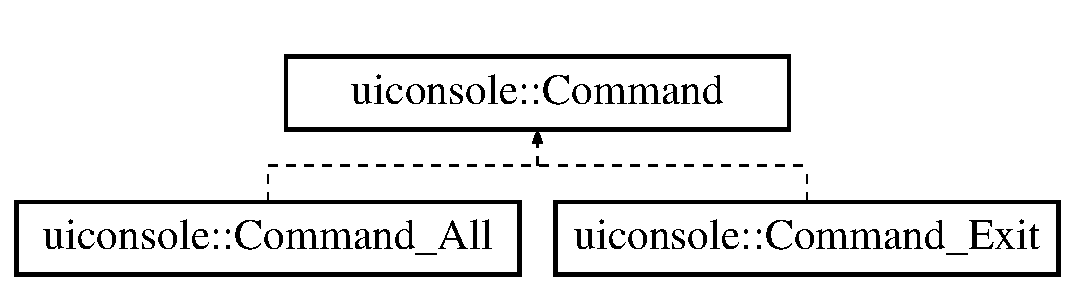
\includegraphics[height=11.000000cm]{dc/df0/classuiconsole_1_1Command}
\end{center}
\end{figure}
\subsection*{Public Member Functions}
\begin{DoxyCompactItemize}
\item 
\hyperlink{classuiconsole_1_1Command_a4f28955b8a36ef1d3b4402b081346060}{Command} (\hyperlink{classUserInterface}{UserInterface} $\ast$\hyperlink{classuiconsole_1_1Command_ab43ed5152860c099f858d62f9f556699}{ui})
\item 
\hyperlink{classuiconsole_1_1Command_a11421d325715cfc8f1e779ef823b3445}{$\sim$Command} ()
\item 
string \hyperlink{classuiconsole_1_1Command_a64d37b0931d5ba0a35d535a6f5a443f3}{get\_\-name} ()
\item 
string \hyperlink{classuiconsole_1_1Command_abcc8cf2d95618e990449e41b510c3fdc}{get\_\-description} ()
\item 
string \hyperlink{classuiconsole_1_1Command_a79b882f32e4ed531f950b0030e2d4998}{get\_\-help} ()
\item 
virtual void \hyperlink{classuiconsole_1_1Command_a5c4d205b1de13a6b3d0db73ddc7ebefa}{run} (vector$<$ string $>$ args)=0
\end{DoxyCompactItemize}
\subsection*{Protected Attributes}
\begin{DoxyCompactItemize}
\item 
\hyperlink{classUserInterface}{UserInterface} $\ast$ \hyperlink{classuiconsole_1_1Command_ab43ed5152860c099f858d62f9f556699}{ui}
\item 
string \hyperlink{classuiconsole_1_1Command_a61eae0502f93a95a9434835f5c72d999}{name}
\item 
string \hyperlink{classuiconsole_1_1Command_ad6dbdcec778315e395a8be8571c3c69d}{description}
\item 
string \hyperlink{classuiconsole_1_1Command_adcc2a70ee67fa5040e6fce1508c490d2}{help}
\end{DoxyCompactItemize}


\subsection{Detailed Description}
Abstract class of console command. 

\subsection{Constructor \& Destructor Documentation}
\hypertarget{classuiconsole_1_1Command_a4f28955b8a36ef1d3b4402b081346060}{
\index{uiconsole::Command@{uiconsole::Command}!Command@{Command}}
\index{Command@{Command}!uiconsole::Command@{uiconsole::Command}}
\subsubsection[{Command}]{\setlength{\rightskip}{0pt plus 5cm}uiconsole::Command::Command (
\begin{DoxyParamCaption}
\item[{{\bf UserInterface} $\ast$}]{ui}
\end{DoxyParamCaption}
)}}
\label{dc/df0/classuiconsole_1_1Command_a4f28955b8a36ef1d3b4402b081346060}
Constructor. 
\begin{DoxyParams}[1]{Parameters}
\mbox{\tt in}  & {\em ui} & pointer to \hyperlink{classUserInterface}{UserInterface}. \\
\hline
\end{DoxyParams}
\hypertarget{classuiconsole_1_1Command_a11421d325715cfc8f1e779ef823b3445}{
\index{uiconsole::Command@{uiconsole::Command}!$\sim$Command@{$\sim$Command}}
\index{$\sim$Command@{$\sim$Command}!uiconsole::Command@{uiconsole::Command}}
\subsubsection[{$\sim$Command}]{\setlength{\rightskip}{0pt plus 5cm}uiconsole::Command::$\sim$Command (
\begin{DoxyParamCaption}
{}
\end{DoxyParamCaption}
)}}
\label{dc/df0/classuiconsole_1_1Command_a11421d325715cfc8f1e779ef823b3445}
Destructor. 

\subsection{Member Function Documentation}
\hypertarget{classuiconsole_1_1Command_abcc8cf2d95618e990449e41b510c3fdc}{
\index{uiconsole::Command@{uiconsole::Command}!get\_\-description@{get\_\-description}}
\index{get\_\-description@{get\_\-description}!uiconsole::Command@{uiconsole::Command}}
\subsubsection[{get\_\-description}]{\setlength{\rightskip}{0pt plus 5cm}string uiconsole::Command::get\_\-description (
\begin{DoxyParamCaption}
{}
\end{DoxyParamCaption}
)}}
\label{dc/df0/classuiconsole_1_1Command_abcc8cf2d95618e990449e41b510c3fdc}
Get description of command. \begin{DoxyReturn}{Returns}
description of command. 
\end{DoxyReturn}
\hypertarget{classuiconsole_1_1Command_a79b882f32e4ed531f950b0030e2d4998}{
\index{uiconsole::Command@{uiconsole::Command}!get\_\-help@{get\_\-help}}
\index{get\_\-help@{get\_\-help}!uiconsole::Command@{uiconsole::Command}}
\subsubsection[{get\_\-help}]{\setlength{\rightskip}{0pt plus 5cm}string uiconsole::Command::get\_\-help (
\begin{DoxyParamCaption}
{}
\end{DoxyParamCaption}
)}}
\label{dc/df0/classuiconsole_1_1Command_a79b882f32e4ed531f950b0030e2d4998}
Get help of command. \begin{DoxyReturn}{Returns}
help of command. 
\end{DoxyReturn}
\hypertarget{classuiconsole_1_1Command_a64d37b0931d5ba0a35d535a6f5a443f3}{
\index{uiconsole::Command@{uiconsole::Command}!get\_\-name@{get\_\-name}}
\index{get\_\-name@{get\_\-name}!uiconsole::Command@{uiconsole::Command}}
\subsubsection[{get\_\-name}]{\setlength{\rightskip}{0pt plus 5cm}string uiconsole::Command::get\_\-name (
\begin{DoxyParamCaption}
{}
\end{DoxyParamCaption}
)}}
\label{dc/df0/classuiconsole_1_1Command_a64d37b0931d5ba0a35d535a6f5a443f3}
Get name of command. \begin{DoxyReturn}{Returns}
name of command. 
\end{DoxyReturn}
\hypertarget{classuiconsole_1_1Command_a5c4d205b1de13a6b3d0db73ddc7ebefa}{
\index{uiconsole::Command@{uiconsole::Command}!run@{run}}
\index{run@{run}!uiconsole::Command@{uiconsole::Command}}
\subsubsection[{run}]{\setlength{\rightskip}{0pt plus 5cm}virtual void uiconsole::Command::run (
\begin{DoxyParamCaption}
\item[{vector$<$ string $>$}]{args}
\end{DoxyParamCaption}
)\hspace{0.3cm}{\ttfamily  \mbox{[}pure virtual\mbox{]}}}}
\label{dc/df0/classuiconsole_1_1Command_a5c4d205b1de13a6b3d0db73ddc7ebefa}
Virtual method called at the execution of command 
\begin{DoxyParams}[1]{Parameters}
\mbox{\tt in}  & {\em args} & Vector of strings used in function \\
\hline
\end{DoxyParams}


Implemented in \hyperlink{classuiconsole_1_1Command__Exit_a83d9528d878c0f3cc8aa26a7c3ebc3c3}{uiconsole::Command\_\-Exit}, \hyperlink{classuiconsole_1_1Command__All_afec181f8031593644a3acca7f5e7fe8f}{uiconsole::Command\_\-All}, \hyperlink{classuiconsole_1_1Command__Print_a42106fe7a7b5ce0c90a5a196c5f8ff42}{uiconsole::Command\_\-Print}, \hyperlink{classuiconsole_1_1Command__Help_a79203580b82e0b17883096640d83e6ff}{uiconsole::Command\_\-Help}, \hyperlink{classuiconsole_1_1Command__Clone_af61cd935a174eaeeec06b98620afe6af}{uiconsole::Command\_\-Clone}, \hyperlink{classuiconsole_1_1Command__Merge_a5d82c5fab7e1f57b885a00eab2cb87b0}{uiconsole::Command\_\-Merge}, \hyperlink{classuiconsole_1_1Command__Exclude_ab2a21ebe3eaf318d9abbbdb89c6fe035}{uiconsole::Command\_\-Exclude}, \hyperlink{classuiconsole_1_1Command__Include_ac4a0f5366a1fbf8d118bde8c5f55e633}{uiconsole::Command\_\-Include}, \hyperlink{classuiconsole_1_1Command__Add_ace9280c73bb3e2a18ace8a4e1ff3ee64}{uiconsole::Command\_\-Add}, and \hyperlink{classuiconsole_1_1Command__Link_a62fc45d4a5aa32b6d2e685f055cec0e6}{uiconsole::Command\_\-Link}.



\subsection{Member Data Documentation}
\hypertarget{classuiconsole_1_1Command_ad6dbdcec778315e395a8be8571c3c69d}{
\index{uiconsole::Command@{uiconsole::Command}!description@{description}}
\index{description@{description}!uiconsole::Command@{uiconsole::Command}}
\subsubsection[{description}]{\setlength{\rightskip}{0pt plus 5cm}string {\bf uiconsole::Command::description}\hspace{0.3cm}{\ttfamily  \mbox{[}protected\mbox{]}}}}
\label{dc/df0/classuiconsole_1_1Command_ad6dbdcec778315e395a8be8571c3c69d}
Description of command. \hypertarget{classuiconsole_1_1Command_adcc2a70ee67fa5040e6fce1508c490d2}{
\index{uiconsole::Command@{uiconsole::Command}!help@{help}}
\index{help@{help}!uiconsole::Command@{uiconsole::Command}}
\subsubsection[{help}]{\setlength{\rightskip}{0pt plus 5cm}string {\bf uiconsole::Command::help}\hspace{0.3cm}{\ttfamily  \mbox{[}protected\mbox{]}}}}
\label{dc/df0/classuiconsole_1_1Command_adcc2a70ee67fa5040e6fce1508c490d2}
Help to the command. \hypertarget{classuiconsole_1_1Command_a61eae0502f93a95a9434835f5c72d999}{
\index{uiconsole::Command@{uiconsole::Command}!name@{name}}
\index{name@{name}!uiconsole::Command@{uiconsole::Command}}
\subsubsection[{name}]{\setlength{\rightskip}{0pt plus 5cm}string {\bf uiconsole::Command::name}\hspace{0.3cm}{\ttfamily  \mbox{[}protected\mbox{]}}}}
\label{dc/df0/classuiconsole_1_1Command_a61eae0502f93a95a9434835f5c72d999}
Name of command. \hypertarget{classuiconsole_1_1Command_ab43ed5152860c099f858d62f9f556699}{
\index{uiconsole::Command@{uiconsole::Command}!ui@{ui}}
\index{ui@{ui}!uiconsole::Command@{uiconsole::Command}}
\subsubsection[{ui}]{\setlength{\rightskip}{0pt plus 5cm}{\bf UserInterface}$\ast$ {\bf uiconsole::Command::ui}\hspace{0.3cm}{\ttfamily  \mbox{[}protected\mbox{]}}}}
\label{dc/df0/classuiconsole_1_1Command_ab43ed5152860c099f858d62f9f556699}
Pointer to user interface object. 

The documentation for this class was generated from the following files:\begin{DoxyCompactItemize}
\item 
src/\hyperlink{commands_8h}{commands.h}\item 
src/\hyperlink{commands_8cpp}{commands.cpp}\end{DoxyCompactItemize}

\hypertarget{classuiconsole_1_1Command__All}{
\section{uiconsole::Command\_\-All Class Reference}
\label{de/dfe/classuiconsole_1_1Command__All}\index{uiconsole::Command\_\-All@{uiconsole::Command\_\-All}}
}


Class of ,,all (s)`` command.  




{\ttfamily \#include $<$commands.h$>$}

Inheritance diagram for uiconsole::Command\_\-All:\begin{figure}[H]
\begin{center}
\leavevmode
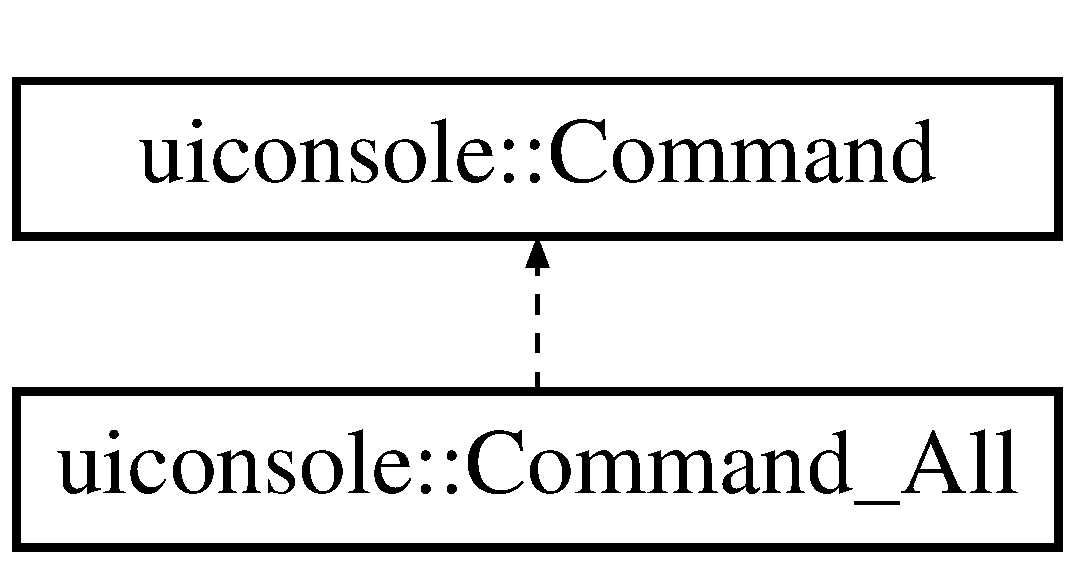
\includegraphics[height=2.000000cm]{de/dfe/classuiconsole_1_1Command__All}
\end{center}
\end{figure}
\subsection*{Public Member Functions}
\begin{DoxyCompactItemize}
\item 
\hyperlink{classuiconsole_1_1Command__All_a8bfd5695c279967bc6667e51a85d2610}{Command\_\-All} (\hyperlink{classUserInterface}{UserInterface} $\ast$\hyperlink{classuiconsole_1_1Command_ab43ed5152860c099f858d62f9f556699}{ui})
\item 
void \hyperlink{classuiconsole_1_1Command__All_afec181f8031593644a3acca7f5e7fe8f}{run} (vector$<$ string $>$ args)
\end{DoxyCompactItemize}


\subsection{Detailed Description}
Class of ,,all (s)`` command. 

\subsection{Constructor \& Destructor Documentation}
\hypertarget{classuiconsole_1_1Command__All_a8bfd5695c279967bc6667e51a85d2610}{
\index{uiconsole::Command\_\-All@{uiconsole::Command\_\-All}!Command\_\-All@{Command\_\-All}}
\index{Command\_\-All@{Command\_\-All}!uiconsole::Command_All@{uiconsole::Command\_\-All}}
\subsubsection[{Command\_\-All}]{\setlength{\rightskip}{0pt plus 5cm}uiconsole::Command\_\-All::Command\_\-All (
\begin{DoxyParamCaption}
\item[{{\bf UserInterface} $\ast$}]{ ui}
\end{DoxyParamCaption}
)}}
\label{de/dfe/classuiconsole_1_1Command__All_a8bfd5695c279967bc6667e51a85d2610}
Constructor. 
\begin{DoxyParams}{Parameters}
\item[\mbox{\tt[in]} {\em ui}]pointer to \hyperlink{classUserInterface}{UserInterface}. \end{DoxyParams}


\subsection{Member Function Documentation}
\hypertarget{classuiconsole_1_1Command__All_afec181f8031593644a3acca7f5e7fe8f}{
\index{uiconsole::Command\_\-All@{uiconsole::Command\_\-All}!run@{run}}
\index{run@{run}!uiconsole::Command_All@{uiconsole::Command\_\-All}}
\subsubsection[{run}]{\setlength{\rightskip}{0pt plus 5cm}void uiconsole::Command\_\-All::run (
\begin{DoxyParamCaption}
\item[{vector$<$ string $>$}]{ args}
\end{DoxyParamCaption}
)\hspace{0.3cm}{\ttfamily  \mbox{[}virtual\mbox{]}}}}
\label{de/dfe/classuiconsole_1_1Command__All_afec181f8031593644a3acca7f5e7fe8f}
Print all objects of a class (s). 
\begin{DoxyParams}{Parameters}
\item[\mbox{\tt[in]} {\em args}]Vector \{\char`\"{}all\char`\"{}, \char`\"{}(s)\char`\"{}\}. \end{DoxyParams}


Implements \hyperlink{classuiconsole_1_1Command_a5c4d205b1de13a6b3d0db73ddc7ebefa}{uiconsole::Command}.



The documentation for this class was generated from the following files:\begin{DoxyCompactItemize}
\item 
src/\hyperlink{commands_8h}{commands.h}\item 
src/\hyperlink{commands_8cpp}{commands.cpp}\end{DoxyCompactItemize}

\hypertarget{classuiconsole_1_1Command__Exit}{
\section{uiconsole::Command\_\-Exit Class Reference}
\label{d5/dd7/classuiconsole_1_1Command__Exit}\index{uiconsole::Command\_\-Exit@{uiconsole::Command\_\-Exit}}
}


Class of ,,exit`` command.  




{\ttfamily \#include $<$commands.h$>$}

Inheritance diagram for uiconsole::Command\_\-Exit:\begin{figure}[H]
\begin{center}
\leavevmode
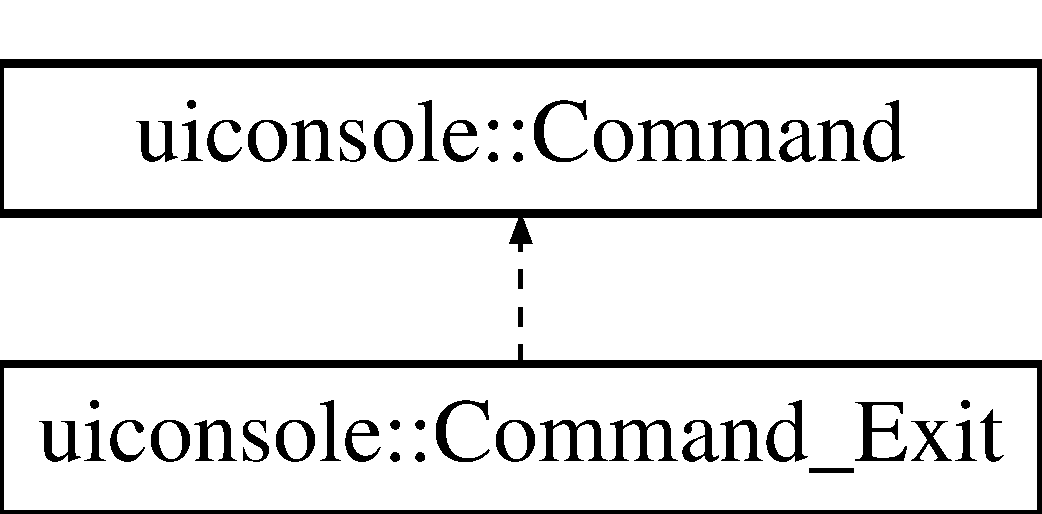
\includegraphics[height=2.000000cm]{d5/dd7/classuiconsole_1_1Command__Exit}
\end{center}
\end{figure}
\subsection*{Public Member Functions}
\begin{DoxyCompactItemize}
\item 
\hyperlink{classuiconsole_1_1Command__Exit_a27f68e3484510c7451417e2babb6b514}{Command\_\-Exit} (\hyperlink{classUserInterface}{UserInterface} $\ast$\hyperlink{classuiconsole_1_1Command_ab43ed5152860c099f858d62f9f556699}{ui})
\item 
void \hyperlink{classuiconsole_1_1Command__Exit_a83d9528d878c0f3cc8aa26a7c3ebc3c3}{run} (vector$<$ string $>$ args)
\end{DoxyCompactItemize}


\subsection{Detailed Description}
Class of ,,exit`` command. 

\subsection{Constructor \& Destructor Documentation}
\hypertarget{classuiconsole_1_1Command__Exit_a27f68e3484510c7451417e2babb6b514}{
\index{uiconsole::Command\_\-Exit@{uiconsole::Command\_\-Exit}!Command\_\-Exit@{Command\_\-Exit}}
\index{Command\_\-Exit@{Command\_\-Exit}!uiconsole::Command_Exit@{uiconsole::Command\_\-Exit}}
\subsubsection[{Command\_\-Exit}]{\setlength{\rightskip}{0pt plus 5cm}uiconsole::Command\_\-Exit::Command\_\-Exit (
\begin{DoxyParamCaption}
\item[{{\bf UserInterface} $\ast$}]{ ui}
\end{DoxyParamCaption}
)}}
\label{d5/dd7/classuiconsole_1_1Command__Exit_a27f68e3484510c7451417e2babb6b514}
Constructor. 
\begin{DoxyParams}{Parameters}
\item[\mbox{\tt[in]} {\em ui}]pointer to \hyperlink{classUserInterface}{UserInterface}. \end{DoxyParams}


\subsection{Member Function Documentation}
\hypertarget{classuiconsole_1_1Command__Exit_a83d9528d878c0f3cc8aa26a7c3ebc3c3}{
\index{uiconsole::Command\_\-Exit@{uiconsole::Command\_\-Exit}!run@{run}}
\index{run@{run}!uiconsole::Command_Exit@{uiconsole::Command\_\-Exit}}
\subsubsection[{run}]{\setlength{\rightskip}{0pt plus 5cm}void uiconsole::Command\_\-Exit::run (
\begin{DoxyParamCaption}
\item[{vector$<$ string $>$}]{ args}
\end{DoxyParamCaption}
)\hspace{0.3cm}{\ttfamily  \mbox{[}virtual\mbox{]}}}}
\label{d5/dd7/classuiconsole_1_1Command__Exit_a83d9528d878c0f3cc8aa26a7c3ebc3c3}
Exit from programm. 
\begin{DoxyParams}{Parameters}
\item[\mbox{\tt[in]} {\em args}]Vector \{\char`\"{}exit\char`\"{}\}. \end{DoxyParams}


Implements \hyperlink{classuiconsole_1_1Command_a5c4d205b1de13a6b3d0db73ddc7ebefa}{uiconsole::Command}.



The documentation for this class was generated from the following files:\begin{DoxyCompactItemize}
\item 
src/\hyperlink{commands_8h}{commands.h}\item 
src/\hyperlink{commands_8cpp}{commands.cpp}\end{DoxyCompactItemize}

\hypertarget{classEvent}{
\section{Event Class Reference}
\label{d5/da5/classEvent}\index{Event@{Event}}
}


Class keeps information about event.  




{\ttfamily \#include $<$event.h$>$}

\subsection*{Public Member Functions}
\begin{DoxyCompactItemize}
\item 
\hyperlink{classEvent_aeec95af5c9bf0410dc9078485dedb2bf}{Event} (\hyperlink{types_8h_ac948e8774f26ce7ea57a66b925e451b9}{id\_\-t} id, string name, time\_\-t begin, time\_\-t end, string description)
\item 
\hyperlink{classEvent_a7704ec01ce91e673885792054214b3d2}{$\sim$Event} ()
\item 
\hyperlink{types_8h_ac948e8774f26ce7ea57a66b925e451b9}{id\_\-t} \hyperlink{classEvent_a526943d871f71a59016637c27da80c23}{get\_\-id} ()
\item 
string \hyperlink{classEvent_a99325a5304e3b73cd4df1f356a185cfc}{get\_\-name} ()
\item 
string \hyperlink{classEvent_a07fdb4a55424b028bfb64db3cea94c07}{get\_\-description} ()
\item 
time\_\-t \hyperlink{classEvent_aa0177bde2838d761774f6e9a50f1e76c}{get\_\-begin} ()
\item 
time\_\-t \hyperlink{classEvent_a25baaf84cc87da4b866f266f946c1d8f}{get\_\-end} ()
\item 
\hyperlink{classGroup}{Group} $\ast$ \hyperlink{classEvent_a5736ec29101416a0358b709c964bf50d}{get\_\-group} ()
\item 
vector$<$ \hyperlink{classCalendar}{Calendar} $\ast$ $>$ $\ast$ \hyperlink{classEvent_ab2329f2021caee686920d5ab2cfa8569}{get\_\-related\_\-calendars} ()
\item 
void \hyperlink{classEvent_a1d59dc31b3358bb9d9d1e75cb735c6ef}{add\_\-related\_\-calendar} (\hyperlink{classCalendar}{Calendar} $\ast$calendar)
\item 
void \hyperlink{classEvent_ac4bc91dab8ca340c58aed7c91a8376a7}{delete\_\-related\_\-calendar} (\hyperlink{classCalendar}{Calendar} $\ast$calendar)
\item 
void \hyperlink{classEvent_a77077d8d27027113b2e20b4374a00a61}{add\_\-person} (class \hyperlink{classPerson}{Person} $\ast$\hyperlink{group__content_8h_ab8664e6fd42f01eeaad084b5e20eb54e}{person}, string \hyperlink{group__content_8h_ab4d38e7365d935f2a5f1403eec29127e}{status})
\item 
void \hyperlink{classEvent_a5e071ee79b9ac9520fa5f26d763ce662}{delete\_\-person} (class \hyperlink{classPerson}{Person} $\ast$\hyperlink{group__content_8h_ab8664e6fd42f01eeaad084b5e20eb54e}{person})
\end{DoxyCompactItemize}


\subsection{Detailed Description}
Class keeps information about event. 

\subsection{Constructor \& Destructor Documentation}
\hypertarget{classEvent_aeec95af5c9bf0410dc9078485dedb2bf}{
\index{Event@{Event}!Event@{Event}}
\index{Event@{Event}!Event@{Event}}
\subsubsection[{Event}]{\setlength{\rightskip}{0pt plus 5cm}Event::Event (
\begin{DoxyParamCaption}
\item[{{\bf id\_\-t}}]{ id, }
\item[{string}]{ name, }
\item[{time\_\-t}]{ begin, }
\item[{time\_\-t}]{ end, }
\item[{string}]{ description}
\end{DoxyParamCaption}
)}}
\label{d5/da5/classEvent_aeec95af5c9bf0410dc9078485dedb2bf}
Constructor. 
\begin{DoxyParams}{Parameters}
\item[\mbox{\tt[in]} {\em id}]Event's identificator in the database. \item[\mbox{\tt[in]} {\em name}]Event's name. \item[\mbox{\tt[in]} {\em begin}]Event's begin time. \item[\mbox{\tt[in]} {\em end}]Event's end time. \item[\mbox{\tt[in]} {\em description}]Event's description. \end{DoxyParams}
\hypertarget{classEvent_a7704ec01ce91e673885792054214b3d2}{
\index{Event@{Event}!$\sim$Event@{$\sim$Event}}
\index{$\sim$Event@{$\sim$Event}!Event@{Event}}
\subsubsection[{$\sim$Event}]{\setlength{\rightskip}{0pt plus 5cm}Event::$\sim$Event (
\begin{DoxyParamCaption}
{}
\end{DoxyParamCaption}
)}}
\label{d5/da5/classEvent_a7704ec01ce91e673885792054214b3d2}
Destructor. 

\subsection{Member Function Documentation}
\hypertarget{classEvent_a77077d8d27027113b2e20b4374a00a61}{
\index{Event@{Event}!add\_\-person@{add\_\-person}}
\index{add\_\-person@{add\_\-person}!Event@{Event}}
\subsubsection[{add\_\-person}]{\setlength{\rightskip}{0pt plus 5cm}void Event::add\_\-person (
\begin{DoxyParamCaption}
\item[{class {\bf Person} $\ast$}]{ person, }
\item[{string}]{ status}
\end{DoxyParamCaption}
)}}
\label{d5/da5/classEvent_a77077d8d27027113b2e20b4374a00a61}
Add person to the event's group. 
\begin{DoxyParams}{Parameters}
\item[\mbox{\tt[in]} {\em person}]\hyperlink{classPerson}{Person} to add. \item[\mbox{\tt[in]} {\em status}]Person's status in the event's group. \end{DoxyParams}
\hypertarget{classEvent_a1d59dc31b3358bb9d9d1e75cb735c6ef}{
\index{Event@{Event}!add\_\-related\_\-calendar@{add\_\-related\_\-calendar}}
\index{add\_\-related\_\-calendar@{add\_\-related\_\-calendar}!Event@{Event}}
\subsubsection[{add\_\-related\_\-calendar}]{\setlength{\rightskip}{0pt plus 5cm}void Event::add\_\-related\_\-calendar (
\begin{DoxyParamCaption}
\item[{{\bf Calendar} $\ast$}]{ calendar}
\end{DoxyParamCaption}
)}}
\label{d5/da5/classEvent_a1d59dc31b3358bb9d9d1e75cb735c6ef}
Add related calendar to event. 
\begin{DoxyParams}{Parameters}
\item[\mbox{\tt[in]} {\em calendar}]\hyperlink{classCalendar}{Calendar} to add. \end{DoxyParams}
\hypertarget{classEvent_a5e071ee79b9ac9520fa5f26d763ce662}{
\index{Event@{Event}!delete\_\-person@{delete\_\-person}}
\index{delete\_\-person@{delete\_\-person}!Event@{Event}}
\subsubsection[{delete\_\-person}]{\setlength{\rightskip}{0pt plus 5cm}void Event::delete\_\-person (
\begin{DoxyParamCaption}
\item[{class {\bf Person} $\ast$}]{ person}
\end{DoxyParamCaption}
)}}
\label{d5/da5/classEvent_a5e071ee79b9ac9520fa5f26d763ce662}
Delete person from the event's group. 
\begin{DoxyParams}{Parameters}
\item[\mbox{\tt[in]} {\em person}]\hyperlink{classPerson}{Person} to delete. \end{DoxyParams}
\hypertarget{classEvent_ac4bc91dab8ca340c58aed7c91a8376a7}{
\index{Event@{Event}!delete\_\-related\_\-calendar@{delete\_\-related\_\-calendar}}
\index{delete\_\-related\_\-calendar@{delete\_\-related\_\-calendar}!Event@{Event}}
\subsubsection[{delete\_\-related\_\-calendar}]{\setlength{\rightskip}{0pt plus 5cm}void Event::delete\_\-related\_\-calendar (
\begin{DoxyParamCaption}
\item[{{\bf Calendar} $\ast$}]{ calendar}
\end{DoxyParamCaption}
)}}
\label{d5/da5/classEvent_ac4bc91dab8ca340c58aed7c91a8376a7}
Delete related calendar from event. 
\begin{DoxyParams}{Parameters}
\item[\mbox{\tt[in]} {\em calendar}]\hyperlink{classCalendar}{Calendar} to delete. \end{DoxyParams}
\hypertarget{classEvent_aa0177bde2838d761774f6e9a50f1e76c}{
\index{Event@{Event}!get\_\-begin@{get\_\-begin}}
\index{get\_\-begin@{get\_\-begin}!Event@{Event}}
\subsubsection[{get\_\-begin}]{\setlength{\rightskip}{0pt plus 5cm}time\_\-t Event::get\_\-begin (
\begin{DoxyParamCaption}
{}
\end{DoxyParamCaption}
)}}
\label{d5/da5/classEvent_aa0177bde2838d761774f6e9a50f1e76c}
Get event's begin time. \begin{DoxyReturn}{Returns}
Event's begin time. 
\end{DoxyReturn}
\hypertarget{classEvent_a07fdb4a55424b028bfb64db3cea94c07}{
\index{Event@{Event}!get\_\-description@{get\_\-description}}
\index{get\_\-description@{get\_\-description}!Event@{Event}}
\subsubsection[{get\_\-description}]{\setlength{\rightskip}{0pt plus 5cm}string Event::get\_\-description (
\begin{DoxyParamCaption}
{}
\end{DoxyParamCaption}
)}}
\label{d5/da5/classEvent_a07fdb4a55424b028bfb64db3cea94c07}
Get event's description. \begin{DoxyReturn}{Returns}
Event's description. 
\end{DoxyReturn}
\hypertarget{classEvent_a25baaf84cc87da4b866f266f946c1d8f}{
\index{Event@{Event}!get\_\-end@{get\_\-end}}
\index{get\_\-end@{get\_\-end}!Event@{Event}}
\subsubsection[{get\_\-end}]{\setlength{\rightskip}{0pt plus 5cm}time\_\-t Event::get\_\-end (
\begin{DoxyParamCaption}
{}
\end{DoxyParamCaption}
)}}
\label{d5/da5/classEvent_a25baaf84cc87da4b866f266f946c1d8f}
Get event's end time. \begin{DoxyReturn}{Returns}
Event's end time. 
\end{DoxyReturn}
\hypertarget{classEvent_a5736ec29101416a0358b709c964bf50d}{
\index{Event@{Event}!get\_\-group@{get\_\-group}}
\index{get\_\-group@{get\_\-group}!Event@{Event}}
\subsubsection[{get\_\-group}]{\setlength{\rightskip}{0pt plus 5cm}{\bf Group} $\ast$ Event::get\_\-group (
\begin{DoxyParamCaption}
{}
\end{DoxyParamCaption}
)}}
\label{d5/da5/classEvent_a5736ec29101416a0358b709c964bf50d}
Get event's group. \begin{DoxyReturn}{Returns}
Event's group. 
\end{DoxyReturn}
\hypertarget{classEvent_a526943d871f71a59016637c27da80c23}{
\index{Event@{Event}!get\_\-id@{get\_\-id}}
\index{get\_\-id@{get\_\-id}!Event@{Event}}
\subsubsection[{get\_\-id}]{\setlength{\rightskip}{0pt plus 5cm}{\bf id\_\-t} Event::get\_\-id (
\begin{DoxyParamCaption}
{}
\end{DoxyParamCaption}
)}}
\label{d5/da5/classEvent_a526943d871f71a59016637c27da80c23}
Get event's identificator. \begin{DoxyReturn}{Returns}
Event's identificator in the database. 
\end{DoxyReturn}
\hypertarget{classEvent_a99325a5304e3b73cd4df1f356a185cfc}{
\index{Event@{Event}!get\_\-name@{get\_\-name}}
\index{get\_\-name@{get\_\-name}!Event@{Event}}
\subsubsection[{get\_\-name}]{\setlength{\rightskip}{0pt plus 5cm}string Event::get\_\-name (
\begin{DoxyParamCaption}
{}
\end{DoxyParamCaption}
)}}
\label{d5/da5/classEvent_a99325a5304e3b73cd4df1f356a185cfc}
Get event's name. \begin{DoxyReturn}{Returns}
Event's name. 
\end{DoxyReturn}
\hypertarget{classEvent_ab2329f2021caee686920d5ab2cfa8569}{
\index{Event@{Event}!get\_\-related\_\-calendars@{get\_\-related\_\-calendars}}
\index{get\_\-related\_\-calendars@{get\_\-related\_\-calendars}!Event@{Event}}
\subsubsection[{get\_\-related\_\-calendars}]{\setlength{\rightskip}{0pt plus 5cm}vector$<$ {\bf Calendar} $\ast$ $>$ $\ast$ Event::get\_\-related\_\-calendars (
\begin{DoxyParamCaption}
{}
\end{DoxyParamCaption}
)}}
\label{d5/da5/classEvent_ab2329f2021caee686920d5ab2cfa8569}
Get event's related calendars. \begin{DoxyReturn}{Returns}
Event's related calendars. 
\end{DoxyReturn}


The documentation for this class was generated from the following files:\begin{DoxyCompactItemize}
\item 
src/\hyperlink{event_8h}{event.h}\item 
src/\hyperlink{event_8cpp}{event.cpp}\end{DoxyCompactItemize}

\hypertarget{classGroup}{
\section{Group Class Reference}
\label{d0/db7/classGroup}\index{Group@{Group}}
}


Class keeps information about group of people.  




{\ttfamily \#include $<$group.h$>$}

\subsection*{Public Member Functions}
\begin{DoxyCompactItemize}
\item 
\hyperlink{classGroup_af95a25f62c49e6aa1e71ef064abc2be4}{Group} (unsigned long long int id, string name, string description)
\item 
\hyperlink{classGroup_a38e2e1f390099856773826609f4e58a1}{Group} (unsigned long long int id, \hyperlink{classGroup}{Group} $\ast$group)
\item 
\hyperlink{classGroup_aed00a22ff227ee2657ae44a5cbcedf7c}{$\sim$Group} ()
\item 
string \hyperlink{classGroup_aab2e4ec29eda3a490dede01eb9411f03}{get\_\-name} ()
\item 
unsigned long long \hyperlink{classGroup_a792a8759e72b90a54f079370d71bdbdb}{get\_\-id} ()
\item 
string \hyperlink{classGroup_ade4eb90fbeb5f50dfb2ccb262cd39ce8}{get\_\-description} ()
\item 
\hyperlink{classCalendar}{Calendar} $\ast$ \hyperlink{classGroup_a10f85a428de5c1215fd7d319bd1a9ca3}{get\_\-calendar} ()
\item 
void \hyperlink{classGroup_a8888e1a6507d004f3b5317fc9a65f005}{add\_\-event} (\hyperlink{classEvent}{Event} $\ast$event)
\item 
void \hyperlink{classGroup_a70b5f6f47818f5d4912926b29faa96bf}{delete\_\-event} (\hyperlink{classEvent}{Event} $\ast$event)
\item 
vector$<$ struct \hyperlink{structGroup__Content__}{Group\_\-Content\_\-} $\ast$ $>$ $\ast$ \hyperlink{classGroup_a8578c69459be6971dd31e76357f934dc}{get\_\-people} ()
\item 
void \hyperlink{classGroup_a2aca17525330aeaf591e0bc243a8149e}{merge\_\-group} (\hyperlink{classGroup}{Group} $\ast$group)
\item 
void \hyperlink{classGroup_a7fccd60929bd2e36db09fe37fffe0548}{exclude\_\-group} (\hyperlink{classGroup}{Group} $\ast$group)
\item 
void \hyperlink{classGroup_ac753fa2674ec19ab156645f978654961}{include\_\-group} (\hyperlink{classGroup}{Group} $\ast$group)
\item 
void \hyperlink{classGroup_afc2080f42e091f6831fd9d80e7b8f0d9}{add\_\-person} (\hyperlink{classPerson}{Person} $\ast$person, string status)
\item 
void \hyperlink{classGroup_ad00847c4219c29fd3b94c6784870b629}{delete\_\-person} (\hyperlink{classPerson}{Person} $\ast$person)
\end{DoxyCompactItemize}


\subsection{Detailed Description}
Class keeps information about group of people. $<$ 

\subsection{Constructor \& Destructor Documentation}
\hypertarget{classGroup_af95a25f62c49e6aa1e71ef064abc2be4}{
\index{Group@{Group}!Group@{Group}}
\index{Group@{Group}!Group@{Group}}
\subsubsection[{Group}]{\setlength{\rightskip}{0pt plus 5cm}Group::Group (
\begin{DoxyParamCaption}
\item[{unsigned long long int}]{id, }
\item[{string}]{name, }
\item[{string}]{description}
\end{DoxyParamCaption}
)}}
\label{d0/db7/classGroup_af95a25f62c49e6aa1e71ef064abc2be4}
Constructor. 
\begin{DoxyParams}[1]{Parameters}
\mbox{\tt in}  & {\em id} & Group's identificator in the database. \\
\hline
\mbox{\tt in}  & {\em name} & Group's name. \\
\hline
\mbox{\tt in}  & {\em description} & Group's description. \\
\hline
\end{DoxyParams}
\hypertarget{classGroup_a38e2e1f390099856773826609f4e58a1}{
\index{Group@{Group}!Group@{Group}}
\index{Group@{Group}!Group@{Group}}
\subsubsection[{Group}]{\setlength{\rightskip}{0pt plus 5cm}Group::Group (
\begin{DoxyParamCaption}
\item[{unsigned long long int}]{id, }
\item[{{\bf Group} $\ast$}]{group}
\end{DoxyParamCaption}
)}}
\label{d0/db7/classGroup_a38e2e1f390099856773826609f4e58a1}
Constructor. 
\begin{DoxyParams}[1]{Parameters}
\mbox{\tt in}  & {\em id} & Group's identificator in the database. \\
\hline
\mbox{\tt in}  & {\em group} & \hyperlink{classGroup}{Group} from which get information. \\
\hline
\end{DoxyParams}
\hypertarget{classGroup_aed00a22ff227ee2657ae44a5cbcedf7c}{
\index{Group@{Group}!$\sim$Group@{$\sim$Group}}
\index{$\sim$Group@{$\sim$Group}!Group@{Group}}
\subsubsection[{$\sim$Group}]{\setlength{\rightskip}{0pt plus 5cm}Group::$\sim$Group (
\begin{DoxyParamCaption}
{}
\end{DoxyParamCaption}
)}}
\label{d0/db7/classGroup_aed00a22ff227ee2657ae44a5cbcedf7c}
Destructor. 

\subsection{Member Function Documentation}
\hypertarget{classGroup_a8888e1a6507d004f3b5317fc9a65f005}{
\index{Group@{Group}!add\_\-event@{add\_\-event}}
\index{add\_\-event@{add\_\-event}!Group@{Group}}
\subsubsection[{add\_\-event}]{\setlength{\rightskip}{0pt plus 5cm}void Group::add\_\-event (
\begin{DoxyParamCaption}
\item[{{\bf Event} $\ast$}]{event}
\end{DoxyParamCaption}
)}}
\label{d0/db7/classGroup_a8888e1a6507d004f3b5317fc9a65f005}
Add event to the group's calendar. 
\begin{DoxyParams}[1]{Parameters}
\mbox{\tt in}  & {\em event} & \hyperlink{classEvent}{Event} to add. \\
\hline
\end{DoxyParams}
\hypertarget{classGroup_afc2080f42e091f6831fd9d80e7b8f0d9}{
\index{Group@{Group}!add\_\-person@{add\_\-person}}
\index{add\_\-person@{add\_\-person}!Group@{Group}}
\subsubsection[{add\_\-person}]{\setlength{\rightskip}{0pt plus 5cm}void Group::add\_\-person (
\begin{DoxyParamCaption}
\item[{{\bf Person} $\ast$}]{person, }
\item[{string}]{status}
\end{DoxyParamCaption}
)}}
\label{d0/db7/classGroup_afc2080f42e091f6831fd9d80e7b8f0d9}
Add person to the group. 
\begin{DoxyParams}{Parameters}
{\em person} & \hyperlink{classPerson}{Person} to add. \\
\hline
{\em status} & Person's status in this group. \\
\hline
\end{DoxyParams}
\hypertarget{classGroup_a70b5f6f47818f5d4912926b29faa96bf}{
\index{Group@{Group}!delete\_\-event@{delete\_\-event}}
\index{delete\_\-event@{delete\_\-event}!Group@{Group}}
\subsubsection[{delete\_\-event}]{\setlength{\rightskip}{0pt plus 5cm}void Group::delete\_\-event (
\begin{DoxyParamCaption}
\item[{{\bf Event} $\ast$}]{event}
\end{DoxyParamCaption}
)}}
\label{d0/db7/classGroup_a70b5f6f47818f5d4912926b29faa96bf}
Delete event from group's calendar. 
\begin{DoxyParams}[1]{Parameters}
\mbox{\tt in}  & {\em event} & \hyperlink{classEvent}{Event} to delete. \\
\hline
\end{DoxyParams}
\hypertarget{classGroup_ad00847c4219c29fd3b94c6784870b629}{
\index{Group@{Group}!delete\_\-person@{delete\_\-person}}
\index{delete\_\-person@{delete\_\-person}!Group@{Group}}
\subsubsection[{delete\_\-person}]{\setlength{\rightskip}{0pt plus 5cm}void Group::delete\_\-person (
\begin{DoxyParamCaption}
\item[{{\bf Person} $\ast$}]{person}
\end{DoxyParamCaption}
)}}
\label{d0/db7/classGroup_ad00847c4219c29fd3b94c6784870b629}
Delete person from group. 
\begin{DoxyParams}{Parameters}
{\em person} & \hyperlink{classPerson}{Person} to delete. \\
\hline
\end{DoxyParams}
\hypertarget{classGroup_a7fccd60929bd2e36db09fe37fffe0548}{
\index{Group@{Group}!exclude\_\-group@{exclude\_\-group}}
\index{exclude\_\-group@{exclude\_\-group}!Group@{Group}}
\subsubsection[{exclude\_\-group}]{\setlength{\rightskip}{0pt plus 5cm}void Group::exclude\_\-group (
\begin{DoxyParamCaption}
\item[{{\bf Group} $\ast$}]{group}
\end{DoxyParamCaption}
)}}
\label{d0/db7/classGroup_a7fccd60929bd2e36db09fe37fffe0548}
Exclude group from this. 
\begin{DoxyParams}{Parameters}
{\em group} & \hyperlink{classGroup}{Group} to exclude. \\
\hline
\end{DoxyParams}
\hypertarget{classGroup_a10f85a428de5c1215fd7d319bd1a9ca3}{
\index{Group@{Group}!get\_\-calendar@{get\_\-calendar}}
\index{get\_\-calendar@{get\_\-calendar}!Group@{Group}}
\subsubsection[{get\_\-calendar}]{\setlength{\rightskip}{0pt plus 5cm}{\bf Calendar} $\ast$ Group::get\_\-calendar (
\begin{DoxyParamCaption}
{}
\end{DoxyParamCaption}
)}}
\label{d0/db7/classGroup_a10f85a428de5c1215fd7d319bd1a9ca3}
Get group's calendar. \begin{DoxyReturn}{Returns}
Group's calendar. 
\end{DoxyReturn}
\hypertarget{classGroup_ade4eb90fbeb5f50dfb2ccb262cd39ce8}{
\index{Group@{Group}!get\_\-description@{get\_\-description}}
\index{get\_\-description@{get\_\-description}!Group@{Group}}
\subsubsection[{get\_\-description}]{\setlength{\rightskip}{0pt plus 5cm}std::string Group::get\_\-description (
\begin{DoxyParamCaption}
{}
\end{DoxyParamCaption}
)}}
\label{d0/db7/classGroup_ade4eb90fbeb5f50dfb2ccb262cd39ce8}
Get group's description. \begin{DoxyReturn}{Returns}
Group's description. 
\end{DoxyReturn}
\hypertarget{classGroup_a792a8759e72b90a54f079370d71bdbdb}{
\index{Group@{Group}!get\_\-id@{get\_\-id}}
\index{get\_\-id@{get\_\-id}!Group@{Group}}
\subsubsection[{get\_\-id}]{\setlength{\rightskip}{0pt plus 5cm}unsigned long long int Group::get\_\-id (
\begin{DoxyParamCaption}
{}
\end{DoxyParamCaption}
)}}
\label{d0/db7/classGroup_a792a8759e72b90a54f079370d71bdbdb}
Get group's identificator. \begin{DoxyReturn}{Returns}
Group's identificator. 
\end{DoxyReturn}
\hypertarget{classGroup_aab2e4ec29eda3a490dede01eb9411f03}{
\index{Group@{Group}!get\_\-name@{get\_\-name}}
\index{get\_\-name@{get\_\-name}!Group@{Group}}
\subsubsection[{get\_\-name}]{\setlength{\rightskip}{0pt plus 5cm}std::string Group::get\_\-name (
\begin{DoxyParamCaption}
{}
\end{DoxyParamCaption}
)}}
\label{d0/db7/classGroup_aab2e4ec29eda3a490dede01eb9411f03}
Get group's name. \begin{DoxyReturn}{Returns}
Group's name. 
\end{DoxyReturn}
\hypertarget{classGroup_a8578c69459be6971dd31e76357f934dc}{
\index{Group@{Group}!get\_\-people@{get\_\-people}}
\index{get\_\-people@{get\_\-people}!Group@{Group}}
\subsubsection[{get\_\-people}]{\setlength{\rightskip}{0pt plus 5cm}std::vector$<$ {\bf Group\_\-Content} $\ast$ $>$ $\ast$ Group::get\_\-people (
\begin{DoxyParamCaption}
{}
\end{DoxyParamCaption}
)}}
\label{d0/db7/classGroup_a8578c69459be6971dd31e76357f934dc}
Get group's people. \begin{DoxyReturn}{Returns}
group's people. 
\end{DoxyReturn}
\hypertarget{classGroup_ac753fa2674ec19ab156645f978654961}{
\index{Group@{Group}!include\_\-group@{include\_\-group}}
\index{include\_\-group@{include\_\-group}!Group@{Group}}
\subsubsection[{include\_\-group}]{\setlength{\rightskip}{0pt plus 5cm}void Group::include\_\-group (
\begin{DoxyParamCaption}
\item[{{\bf Group} $\ast$}]{group}
\end{DoxyParamCaption}
)}}
\label{d0/db7/classGroup_ac753fa2674ec19ab156645f978654961}
Select includes in group. 
\begin{DoxyParams}{Parameters}
{\em group} & \hyperlink{classGroup}{Group} to include. \\
\hline
\end{DoxyParams}
\hypertarget{classGroup_a2aca17525330aeaf591e0bc243a8149e}{
\index{Group@{Group}!merge\_\-group@{merge\_\-group}}
\index{merge\_\-group@{merge\_\-group}!Group@{Group}}
\subsubsection[{merge\_\-group}]{\setlength{\rightskip}{0pt plus 5cm}void Group::merge\_\-group (
\begin{DoxyParamCaption}
\item[{{\bf Group} $\ast$}]{group}
\end{DoxyParamCaption}
)}}
\label{d0/db7/classGroup_a2aca17525330aeaf591e0bc243a8149e}
Merge group with this. 
\begin{DoxyParams}{Parameters}
{\em group} & \hyperlink{classGroup}{Group} to merge. \\
\hline
\end{DoxyParams}


The documentation for this class was generated from the following files:\begin{DoxyCompactItemize}
\item 
src/\hyperlink{group_8h}{group.h}\item 
src/\hyperlink{group_8cpp}{group.cpp}\end{DoxyCompactItemize}

\hypertarget{structGroup__Content}{
\section{Group\_\-Content Struct Reference}
\label{d2/d04/structGroup__Content}\index{Group\_\-Content@{Group\_\-Content}}
}


\subsection{Detailed Description}
people and groups. 

The documentation for this struct was generated from the following file:\begin{DoxyCompactItemize}
\item 
src/\hyperlink{group__content_8h}{group\_\-content.h}\end{DoxyCompactItemize}

\hypertarget{structGroup__Content__}{
\section{Group\_\-Content\_\- Struct Reference}
\label{d9/d96/structGroup__Content__}\index{Group\_\-Content\_\-@{Group\_\-Content\_\-}}
}


{\ttfamily \#include $<$group\_\-content.h$>$}

\subsection*{Public Attributes}
\begin{DoxyCompactItemize}
\item 
class \hyperlink{classGroup}{Group} $\ast$ \hyperlink{structGroup__Content___aff21edda2f29d751074e18d71dbbc1e4}{group}
\item 
class \hyperlink{classPerson}{Person} $\ast$ \hyperlink{structGroup__Content___a71f0da92a56d69af4275f011d443fb09}{person}
\item 
string \hyperlink{structGroup__Content___acd55c0cc8ecafe72189cc849c07da3b3}{status}
\end{DoxyCompactItemize}


\subsection{Member Data Documentation}
\hypertarget{structGroup__Content___aff21edda2f29d751074e18d71dbbc1e4}{
\index{Group\_\-Content\_\-@{Group\_\-Content\_\-}!group@{group}}
\index{group@{group}!Group_Content_@{Group\_\-Content\_\-}}
\subsubsection[{group}]{\setlength{\rightskip}{0pt plus 5cm}class {\bf Group}$\ast$ {\bf Group\_\-Content\_\-::group}}}
\label{d9/d96/structGroup__Content___aff21edda2f29d751074e18d71dbbc1e4}
\hyperlink{classGroup}{Group}. \hypertarget{structGroup__Content___a71f0da92a56d69af4275f011d443fb09}{
\index{Group\_\-Content\_\-@{Group\_\-Content\_\-}!person@{person}}
\index{person@{person}!Group_Content_@{Group\_\-Content\_\-}}
\subsubsection[{person}]{\setlength{\rightskip}{0pt plus 5cm}class {\bf Person}$\ast$ {\bf Group\_\-Content\_\-::person}}}
\label{d9/d96/structGroup__Content___a71f0da92a56d69af4275f011d443fb09}
\hyperlink{classPerson}{Person}. \hypertarget{structGroup__Content___acd55c0cc8ecafe72189cc849c07da3b3}{
\index{Group\_\-Content\_\-@{Group\_\-Content\_\-}!status@{status}}
\index{status@{status}!Group_Content_@{Group\_\-Content\_\-}}
\subsubsection[{status}]{\setlength{\rightskip}{0pt plus 5cm}string {\bf Group\_\-Content\_\-::status}}}
\label{d9/d96/structGroup__Content___acd55c0cc8ecafe72189cc849c07da3b3}
Person's status in this group. 

The documentation for this struct was generated from the following file:\begin{DoxyCompactItemize}
\item 
src/\hyperlink{group__content_8h}{group\_\-content.h}\end{DoxyCompactItemize}

\hypertarget{classPerson}{
\section{Person Class Reference}
\label{d1/d63/classPerson}\index{Person@{Person}}
}


Class keeps person unique data.  




{\ttfamily \#include $<$person.h$>$}

\subsection*{Public Types}
\begin{DoxyCompactItemize}
\item 
enum \hyperlink{classPerson_a328ea8d2e8c2674688c7f944fab70b6b}{Sex} \{ \hyperlink{classPerson_a328ea8d2e8c2674688c7f944fab70b6ba16691f7cc6595f87b71d9b43ad23fcb4}{MALE}, 
\hyperlink{classPerson_a328ea8d2e8c2674688c7f944fab70b6ba8ee21010fb2d8e8794ef72be368da064}{FEMALE}
 \}
\end{DoxyCompactItemize}
\subsection*{Public Member Functions}
\begin{DoxyCompactItemize}
\item 
\hyperlink{classPerson_a1b0a164e39923dc6a7bd37a075dceda7}{Person} (\hyperlink{types_8h_a0b60c08a3ab1435cccc5643d32d8ccee}{id\_\-type} id, std::string name, std::string surname, bool female, time\_\-t birthday)
\item 
\hyperlink{classPerson_a700ffd693321c5fe6880262acf43d4da}{$\sim$Person} ()
\item 
\hyperlink{types_8h_a0b60c08a3ab1435cccc5643d32d8ccee}{id\_\-type} \hyperlink{classPerson_addbe4758044124636fb0f9d3094c6fcb}{get\_\-id} ()
\item 
std::string \hyperlink{classPerson_a1837ca2f4ba804aeee2a70c1a1fdd468}{get\_\-name} ()
\item 
std::string \hyperlink{classPerson_aad33f79ec5c96aa3ab30c9c4c989fb4b}{get\_\-surname} ()
\item 
bool \hyperlink{classPerson_a8bfe5b0c264f051b85812c692691e277}{is\_\-female} ()
\item 
time\_\-t \hyperlink{classPerson_aec14dd73ca58227cc70c4ba3a5065d02}{birthday} ()
\item 
std::vector$<$ \hyperlink{structGroup__Content}{Group\_\-Content} $\ast$ $>$ $\ast$ \hyperlink{classPerson_a24cd3ad56c42c1cd34505b1094e6e7d5}{get\_\-groups} ()
\item 
void \hyperlink{classPerson_aa17159e6bb16f2a42a1c4bcae08ae903}{add\_\-group} (\hyperlink{structGroup__Content}{Group\_\-Content} $\ast$\hyperlink{group__content_8h_a27517aa1480ab2d9bfe5d62e693b33eb}{group})
\item 
void \hyperlink{classPerson_a93dfe7e17e0316b1f7dddebf5fd3f7ce}{delete\_\-group} (\hyperlink{classGroup}{Group} $\ast$\hyperlink{group__content_8h_a27517aa1480ab2d9bfe5d62e693b33eb}{group})
\item 
\hyperlink{classCalendar}{Calendar} $\ast$ \hyperlink{classPerson_abaaac95db5394d3ad78ad08221b1d231}{get\_\-calendar} ()
\item 
void \hyperlink{classPerson_a57689e959d613756a806e5d32654d3e8}{add\_\-event} (\hyperlink{classEvent}{Event} $\ast$event, std::string \hyperlink{group__content_8h_ab4d38e7365d935f2a5f1403eec29127e}{status})
\item 
void \hyperlink{classPerson_ab788997b3b66a72e51f924d416029ff5}{delete\_\-event} (\hyperlink{classEvent}{Event} $\ast$event)
\end{DoxyCompactItemize}


\subsection{Detailed Description}
Class keeps person unique data. 

\subsection{Member Enumeration Documentation}
\hypertarget{classPerson_a328ea8d2e8c2674688c7f944fab70b6b}{
\index{Person@{Person}!Sex@{Sex}}
\index{Sex@{Sex}!Person@{Person}}
\subsubsection[{Sex}]{\setlength{\rightskip}{0pt plus 5cm}enum {\bf Person::Sex}}}
\label{d1/d63/classPerson_a328ea8d2e8c2674688c7f944fab70b6b}
enum of sex \begin{Desc}
\item[Enumerator: ]\par
\begin{description}
\index{MALE@{MALE}!Person@{Person}}\index{Person@{Person}!MALE@{MALE}}\item[{\em 
\hypertarget{classPerson_a328ea8d2e8c2674688c7f944fab70b6ba16691f7cc6595f87b71d9b43ad23fcb4}{
MALE}
\label{d1/d63/classPerson_a328ea8d2e8c2674688c7f944fab70b6ba16691f7cc6595f87b71d9b43ad23fcb4}
}]\index{FEMALE@{FEMALE}!Person@{Person}}\index{Person@{Person}!FEMALE@{FEMALE}}\item[{\em 
\hypertarget{classPerson_a328ea8d2e8c2674688c7f944fab70b6ba8ee21010fb2d8e8794ef72be368da064}{
FEMALE}
\label{d1/d63/classPerson_a328ea8d2e8c2674688c7f944fab70b6ba8ee21010fb2d8e8794ef72be368da064}
}]\end{description}
\end{Desc}



\subsection{Constructor \& Destructor Documentation}
\hypertarget{classPerson_a1b0a164e39923dc6a7bd37a075dceda7}{
\index{Person@{Person}!Person@{Person}}
\index{Person@{Person}!Person@{Person}}
\subsubsection[{Person}]{\setlength{\rightskip}{0pt plus 5cm}Person::Person (
\begin{DoxyParamCaption}
\item[{{\bf id\_\-type}}]{ id, }
\item[{std::string}]{ name, }
\item[{std::string}]{ surname, }
\item[{bool}]{ female, }
\item[{time\_\-t}]{ birthday}
\end{DoxyParamCaption}
)}}
\label{d1/d63/classPerson_a1b0a164e39923dc6a7bd37a075dceda7}
Constructor. 
\begin{DoxyParams}{Parameters}
\item[\mbox{\tt[in]} {\em id}]Person's identificator. \item[\mbox{\tt[in]} {\em name}]Person's name. \item[\mbox{\tt[in]} {\em surname}]Person's surname. \item[\mbox{\tt[in]} {\em female}]Person's sex. \item[\mbox{\tt[in]} {\em birthday}]Person's birthday. \end{DoxyParams}
\hypertarget{classPerson_a700ffd693321c5fe6880262acf43d4da}{
\index{Person@{Person}!$\sim$Person@{$\sim$Person}}
\index{$\sim$Person@{$\sim$Person}!Person@{Person}}
\subsubsection[{$\sim$Person}]{\setlength{\rightskip}{0pt plus 5cm}Person::$\sim$Person (
\begin{DoxyParamCaption}
{}
\end{DoxyParamCaption}
)}}
\label{d1/d63/classPerson_a700ffd693321c5fe6880262acf43d4da}
Destructor. 

\subsection{Member Function Documentation}
\hypertarget{classPerson_a57689e959d613756a806e5d32654d3e8}{
\index{Person@{Person}!add\_\-event@{add\_\-event}}
\index{add\_\-event@{add\_\-event}!Person@{Person}}
\subsubsection[{add\_\-event}]{\setlength{\rightskip}{0pt plus 5cm}void Person::add\_\-event (
\begin{DoxyParamCaption}
\item[{{\bf Event} $\ast$}]{ event, }
\item[{std::string}]{ status}
\end{DoxyParamCaption}
)}}
\label{d1/d63/classPerson_a57689e959d613756a806e5d32654d3e8}
Add event to the person's calendar. 
\begin{DoxyParams}{Parameters}
\item[\mbox{\tt[in]} {\em event}]event. \item[\mbox{\tt[in]} {\em status}]person's status in this event. \end{DoxyParams}
\hypertarget{classPerson_aa17159e6bb16f2a42a1c4bcae08ae903}{
\index{Person@{Person}!add\_\-group@{add\_\-group}}
\index{add\_\-group@{add\_\-group}!Person@{Person}}
\subsubsection[{add\_\-group}]{\setlength{\rightskip}{0pt plus 5cm}void Person::add\_\-group (
\begin{DoxyParamCaption}
\item[{{\bf Group\_\-Content} $\ast$}]{ group}
\end{DoxyParamCaption}
)}}
\label{d1/d63/classPerson_aa17159e6bb16f2a42a1c4bcae08ae903}
Add group. 
\begin{DoxyParams}{Parameters}
\item[\mbox{\tt[in]} {\em group}]group. \end{DoxyParams}
\hypertarget{classPerson_aec14dd73ca58227cc70c4ba3a5065d02}{
\index{Person@{Person}!birthday@{birthday}}
\index{birthday@{birthday}!Person@{Person}}
\subsubsection[{birthday}]{\setlength{\rightskip}{0pt plus 5cm}time\_\-t Person::birthday (
\begin{DoxyParamCaption}
{}
\end{DoxyParamCaption}
)}}
\label{d1/d63/classPerson_aec14dd73ca58227cc70c4ba3a5065d02}
Get birthday of person. \begin{DoxyReturn}{Returns}
person's birthday. 
\end{DoxyReturn}
\hypertarget{classPerson_ab788997b3b66a72e51f924d416029ff5}{
\index{Person@{Person}!delete\_\-event@{delete\_\-event}}
\index{delete\_\-event@{delete\_\-event}!Person@{Person}}
\subsubsection[{delete\_\-event}]{\setlength{\rightskip}{0pt plus 5cm}void Person::delete\_\-event (
\begin{DoxyParamCaption}
\item[{{\bf Event} $\ast$}]{ event}
\end{DoxyParamCaption}
)}}
\label{d1/d63/classPerson_ab788997b3b66a72e51f924d416029ff5}
Delete event from the person's calendar. 
\begin{DoxyParams}{Parameters}
\item[\mbox{\tt[in]} {\em event}]event. \end{DoxyParams}
\hypertarget{classPerson_a93dfe7e17e0316b1f7dddebf5fd3f7ce}{
\index{Person@{Person}!delete\_\-group@{delete\_\-group}}
\index{delete\_\-group@{delete\_\-group}!Person@{Person}}
\subsubsection[{delete\_\-group}]{\setlength{\rightskip}{0pt plus 5cm}void Person::delete\_\-group (
\begin{DoxyParamCaption}
\item[{{\bf Group} $\ast$}]{ group}
\end{DoxyParamCaption}
)}}
\label{d1/d63/classPerson_a93dfe7e17e0316b1f7dddebf5fd3f7ce}
Delete group. 
\begin{DoxyParams}{Parameters}
\item[\mbox{\tt[in]} {\em group}]group. \end{DoxyParams}
\hypertarget{classPerson_abaaac95db5394d3ad78ad08221b1d231}{
\index{Person@{Person}!get\_\-calendar@{get\_\-calendar}}
\index{get\_\-calendar@{get\_\-calendar}!Person@{Person}}
\subsubsection[{get\_\-calendar}]{\setlength{\rightskip}{0pt plus 5cm}{\bf Calendar} $\ast$ Person::get\_\-calendar (
\begin{DoxyParamCaption}
{}
\end{DoxyParamCaption}
)}}
\label{d1/d63/classPerson_abaaac95db5394d3ad78ad08221b1d231}
Get calendar of person. \begin{DoxyReturn}{Returns}
\mbox{[}in\mbox{]} calendar calendar. 
\end{DoxyReturn}
\hypertarget{classPerson_a24cd3ad56c42c1cd34505b1094e6e7d5}{
\index{Person@{Person}!get\_\-groups@{get\_\-groups}}
\index{get\_\-groups@{get\_\-groups}!Person@{Person}}
\subsubsection[{get\_\-groups}]{\setlength{\rightskip}{0pt plus 5cm}std::vector$<$ {\bf Group\_\-Content} $\ast$ $>$ $\ast$ Person::get\_\-groups (
\begin{DoxyParamCaption}
{}
\end{DoxyParamCaption}
)}}
\label{d1/d63/classPerson_a24cd3ad56c42c1cd34505b1094e6e7d5}
Get groups of person. \begin{DoxyReturn}{Returns}
vector of person's groups. 
\end{DoxyReturn}
\hypertarget{classPerson_addbe4758044124636fb0f9d3094c6fcb}{
\index{Person@{Person}!get\_\-id@{get\_\-id}}
\index{get\_\-id@{get\_\-id}!Person@{Person}}
\subsubsection[{get\_\-id}]{\setlength{\rightskip}{0pt plus 5cm}{\bf id\_\-type} Person::get\_\-id (
\begin{DoxyParamCaption}
{}
\end{DoxyParamCaption}
)}}
\label{d1/d63/classPerson_addbe4758044124636fb0f9d3094c6fcb}
Get id of person in database. \begin{DoxyReturn}{Returns}
id of person. 
\end{DoxyReturn}
\hypertarget{classPerson_a1837ca2f4ba804aeee2a70c1a1fdd468}{
\index{Person@{Person}!get\_\-name@{get\_\-name}}
\index{get\_\-name@{get\_\-name}!Person@{Person}}
\subsubsection[{get\_\-name}]{\setlength{\rightskip}{0pt plus 5cm}std::string Person::get\_\-name (
\begin{DoxyParamCaption}
{}
\end{DoxyParamCaption}
)}}
\label{d1/d63/classPerson_a1837ca2f4ba804aeee2a70c1a1fdd468}
Get name of person. \begin{DoxyReturn}{Returns}
name of person. 
\end{DoxyReturn}
\hypertarget{classPerson_aad33f79ec5c96aa3ab30c9c4c989fb4b}{
\index{Person@{Person}!get\_\-surname@{get\_\-surname}}
\index{get\_\-surname@{get\_\-surname}!Person@{Person}}
\subsubsection[{get\_\-surname}]{\setlength{\rightskip}{0pt plus 5cm}std::string Person::get\_\-surname (
\begin{DoxyParamCaption}
{}
\end{DoxyParamCaption}
)}}
\label{d1/d63/classPerson_aad33f79ec5c96aa3ab30c9c4c989fb4b}
Get surname of person. \begin{DoxyReturn}{Returns}
surname of person. 
\end{DoxyReturn}
\hypertarget{classPerson_a8bfe5b0c264f051b85812c692691e277}{
\index{Person@{Person}!is\_\-female@{is\_\-female}}
\index{is\_\-female@{is\_\-female}!Person@{Person}}
\subsubsection[{is\_\-female}]{\setlength{\rightskip}{0pt plus 5cm}bool Person::is\_\-female (
\begin{DoxyParamCaption}
{}
\end{DoxyParamCaption}
)}}
\label{d1/d63/classPerson_a8bfe5b0c264f051b85812c692691e277}
Get sex of person. \begin{DoxyReturn}{Returns}
person's sex. 
\end{DoxyReturn}


The documentation for this class was generated from the following files:\begin{DoxyCompactItemize}
\item 
src/\hyperlink{person_8h}{person.h}\item 
src/\hyperlink{person_8cpp}{person.cpp}\end{DoxyCompactItemize}

\hypertarget{classUserInterface}{
\section{UserInterface Class Reference}
\label{df/de1/classUserInterface}\index{UserInterface@{UserInterface}}
}


Class provides user interface.  




{\ttfamily \#include $<$userinterface.h$>$}

\subsection*{Public Member Functions}
\begin{DoxyCompactItemize}
\item 
\hyperlink{classUserInterface_a72d625f6d41876d679ed067e0f273ed8}{UserInterface} (vector$<$ \hyperlink{classPerson}{Person} $\ast$ $>$ $\ast$\hyperlink{classUserInterface_a3d0914e9d2ba661bc3691397c695287e}{people}, vector$<$ \hyperlink{classGroup}{Group} $\ast$ $>$ $\ast$\hyperlink{classUserInterface_a12676e629660c43c63eb5b01c5c19bc3}{groups}, vector$<$ \hyperlink{classEvent}{Event} $\ast$ $>$ $\ast$\hyperlink{classUserInterface_ae3370dc0d02c19b4b1cc7c47221c2bfa}{events}, vector$<$ \hyperlink{classCalendar}{Calendar} $\ast$ $>$ $\ast$\hyperlink{classUserInterface_abd1f3233d3e666415f6cdf8458b50faa}{calendars})
\item 
\hyperlink{classUserInterface_ae588b2ff1711a016dd4c6fc5002c0841}{$\sim$UserInterface} ()
\item 
void \hyperlink{classUserInterface_ac1cead6c14db26f88802ea035fb59bd9}{listen} ()
\item 
void \hyperlink{classUserInterface_a396eb29856a6afc91bc0e0eef1de2df7}{exit} ()
\item 
void \hyperlink{classUserInterface_a36513fcf018fafc53726cf610f46571f}{set\_\-format} (enum \hyperlink{userinterface_8h_a5a0e707f53d6c5632b2fb5ffd2d22a11}{default\_\-format} format)
\item 
enum \hyperlink{userinterface_8h_a5a0e707f53d6c5632b2fb5ffd2d22a11}{default\_\-format} \hyperlink{classUserInterface_ad543750a7accc0c4825e02a93fda1909}{get\_\-format} ()
\item 
void \hyperlink{classUserInterface_a9373bc1aedbdc68905942bcb7c6a8fd3}{format} (time\_\-t time)
\item 
void \hyperlink{classUserInterface_a41c109a7e042b44dc98a1250681fc684}{format\_\-ASCII} (time\_\-t time)
\item 
void \hyperlink{classUserInterface_a45a7ad6cca95218631d8c6fbe49362e2}{print\_\-person} (\hyperlink{classPerson}{Person} $\ast$\hyperlink{group__content_8h_ab8664e6fd42f01eeaad084b5e20eb54e}{person})
\item 
void \hyperlink{classUserInterface_a31424519b61f71584a4a5196c6632beb}{print\_\-group} (\hyperlink{classGroup}{Group} $\ast$\hyperlink{group__content_8h_a27517aa1480ab2d9bfe5d62e693b33eb}{group})
\item 
void \hyperlink{classUserInterface_aca628f5a276b39ff4346e2150b419590}{print\_\-event} (\hyperlink{classEvent}{Event} $\ast$event)
\item 
void \hyperlink{classUserInterface_aca95eaf06d053b4ac267e94ccb84e501}{print\_\-calendar} (\hyperlink{classCalendar}{Calendar} $\ast$calendar)
\end{DoxyCompactItemize}
\subsection*{Public Attributes}
\begin{DoxyCompactItemize}
\item 
vector$<$ \hyperlink{classPerson}{Person} $\ast$ $>$ $\ast$ \hyperlink{classUserInterface_a3d0914e9d2ba661bc3691397c695287e}{people}
\item 
vector$<$ \hyperlink{classGroup}{Group} $\ast$ $>$ $\ast$ \hyperlink{classUserInterface_a12676e629660c43c63eb5b01c5c19bc3}{groups}
\item 
vector$<$ \hyperlink{classEvent}{Event} $\ast$ $>$ $\ast$ \hyperlink{classUserInterface_ae3370dc0d02c19b4b1cc7c47221c2bfa}{events}
\item 
vector$<$ \hyperlink{classCalendar}{Calendar} $\ast$ $>$ $\ast$ \hyperlink{classUserInterface_abd1f3233d3e666415f6cdf8458b50faa}{calendars}
\end{DoxyCompactItemize}


\subsection{Detailed Description}
Class provides user interface. 

\subsection{Constructor \& Destructor Documentation}
\hypertarget{classUserInterface_a72d625f6d41876d679ed067e0f273ed8}{
\index{UserInterface@{UserInterface}!UserInterface@{UserInterface}}
\index{UserInterface@{UserInterface}!UserInterface@{UserInterface}}
\subsubsection[{UserInterface}]{\setlength{\rightskip}{0pt plus 5cm}UserInterface::UserInterface (
\begin{DoxyParamCaption}
\item[{vector$<$ {\bf Person} $\ast$ $>$ $\ast$}]{ people, }
\item[{vector$<$ {\bf Group} $\ast$ $>$ $\ast$}]{ groups, }
\item[{vector$<$ {\bf Event} $\ast$ $>$ $\ast$}]{ events, }
\item[{vector$<$ {\bf Calendar} $\ast$ $>$ $\ast$}]{ calendars}
\end{DoxyParamCaption}
)}}
\label{df/de1/classUserInterface_a72d625f6d41876d679ed067e0f273ed8}
Constructor 
\begin{DoxyParams}{Parameters}
\item[\mbox{\tt[in]} {\em people}]All people objects in the programm. \item[\mbox{\tt[in]} {\em groups}]All groups objects. \item[\mbox{\tt[in]} {\em events}]All events objects. \item[\mbox{\tt[in]} {\em calendars}]All calendars objects. \end{DoxyParams}
\hypertarget{classUserInterface_ae588b2ff1711a016dd4c6fc5002c0841}{
\index{UserInterface@{UserInterface}!$\sim$UserInterface@{$\sim$UserInterface}}
\index{$\sim$UserInterface@{$\sim$UserInterface}!UserInterface@{UserInterface}}
\subsubsection[{$\sim$UserInterface}]{\setlength{\rightskip}{0pt plus 5cm}UserInterface::$\sim$UserInterface (
\begin{DoxyParamCaption}
{}
\end{DoxyParamCaption}
)}}
\label{df/de1/classUserInterface_ae588b2ff1711a016dd4c6fc5002c0841}
Destructor 

\subsection{Member Function Documentation}
\hypertarget{classUserInterface_a396eb29856a6afc91bc0e0eef1de2df7}{
\index{UserInterface@{UserInterface}!exit@{exit}}
\index{exit@{exit}!UserInterface@{UserInterface}}
\subsubsection[{exit}]{\setlength{\rightskip}{0pt plus 5cm}void UserInterface::exit (
\begin{DoxyParamCaption}
{}
\end{DoxyParamCaption}
)}}
\label{df/de1/classUserInterface_a396eb29856a6afc91bc0e0eef1de2df7}
Exit from interactive command line mode. \hypertarget{classUserInterface_a9373bc1aedbdc68905942bcb7c6a8fd3}{
\index{UserInterface@{UserInterface}!format@{format}}
\index{format@{format}!UserInterface@{UserInterface}}
\subsubsection[{format}]{\setlength{\rightskip}{0pt plus 5cm}void UserInterface::format (
\begin{DoxyParamCaption}
\item[{time\_\-t}]{ time}
\end{DoxyParamCaption}
)}}
\label{df/de1/classUserInterface_a9373bc1aedbdc68905942bcb7c6a8fd3}
Print time in default format. 
\begin{DoxyParams}{Parameters}
\item[\mbox{\tt[in]} {\em time}]Time to print. \end{DoxyParams}
\hypertarget{classUserInterface_a41c109a7e042b44dc98a1250681fc684}{
\index{UserInterface@{UserInterface}!format\_\-ASCII@{format\_\-ASCII}}
\index{format\_\-ASCII@{format\_\-ASCII}!UserInterface@{UserInterface}}
\subsubsection[{format\_\-ASCII}]{\setlength{\rightskip}{0pt plus 5cm}void UserInterface::format\_\-ASCII (
\begin{DoxyParamCaption}
\item[{time\_\-t}]{ time}
\end{DoxyParamCaption}
)}}
\label{df/de1/classUserInterface_a41c109a7e042b44dc98a1250681fc684}
Print time in ASCII time format. 
\begin{DoxyParams}{Parameters}
\item[\mbox{\tt[in]} {\em time}]Time to print. \end{DoxyParams}
\hypertarget{classUserInterface_ad543750a7accc0c4825e02a93fda1909}{
\index{UserInterface@{UserInterface}!get\_\-format@{get\_\-format}}
\index{get\_\-format@{get\_\-format}!UserInterface@{UserInterface}}
\subsubsection[{get\_\-format}]{\setlength{\rightskip}{0pt plus 5cm}enum {\bf default\_\-format} UserInterface::get\_\-format (
\begin{DoxyParamCaption}
{}
\end{DoxyParamCaption}
)}}
\label{df/de1/classUserInterface_ad543750a7accc0c4825e02a93fda1909}
Get default time format. \begin{DoxyReturn}{Returns}
Default type of time format. 
\end{DoxyReturn}
\hypertarget{classUserInterface_ac1cead6c14db26f88802ea035fb59bd9}{
\index{UserInterface@{UserInterface}!listen@{listen}}
\index{listen@{listen}!UserInterface@{UserInterface}}
\subsubsection[{listen}]{\setlength{\rightskip}{0pt plus 5cm}void UserInterface::listen (
\begin{DoxyParamCaption}
{}
\end{DoxyParamCaption}
)}}
\label{df/de1/classUserInterface_ac1cead6c14db26f88802ea035fb59bd9}
Interactive command line mode. \hypertarget{classUserInterface_aca95eaf06d053b4ac267e94ccb84e501}{
\index{UserInterface@{UserInterface}!print\_\-calendar@{print\_\-calendar}}
\index{print\_\-calendar@{print\_\-calendar}!UserInterface@{UserInterface}}
\subsubsection[{print\_\-calendar}]{\setlength{\rightskip}{0pt plus 5cm}void UserInterface::print\_\-calendar (
\begin{DoxyParamCaption}
\item[{{\bf Calendar} $\ast$}]{ calendar}
\end{DoxyParamCaption}
)}}
\label{df/de1/classUserInterface_aca95eaf06d053b4ac267e94ccb84e501}
Print calendar's information. 
\begin{DoxyParams}{Parameters}
\item[\mbox{\tt[in]} {\em calendar}]\hyperlink{classCalendar}{Calendar} to print. \end{DoxyParams}
\hypertarget{classUserInterface_aca628f5a276b39ff4346e2150b419590}{
\index{UserInterface@{UserInterface}!print\_\-event@{print\_\-event}}
\index{print\_\-event@{print\_\-event}!UserInterface@{UserInterface}}
\subsubsection[{print\_\-event}]{\setlength{\rightskip}{0pt plus 5cm}void UserInterface::print\_\-event (
\begin{DoxyParamCaption}
\item[{{\bf Event} $\ast$}]{ event}
\end{DoxyParamCaption}
)}}
\label{df/de1/classUserInterface_aca628f5a276b39ff4346e2150b419590}
Print event's information. 
\begin{DoxyParams}{Parameters}
\item[\mbox{\tt[in]} {\em event}]\hyperlink{classEvent}{Event} to print. \end{DoxyParams}
\hypertarget{classUserInterface_a31424519b61f71584a4a5196c6632beb}{
\index{UserInterface@{UserInterface}!print\_\-group@{print\_\-group}}
\index{print\_\-group@{print\_\-group}!UserInterface@{UserInterface}}
\subsubsection[{print\_\-group}]{\setlength{\rightskip}{0pt plus 5cm}void UserInterface::print\_\-group (
\begin{DoxyParamCaption}
\item[{{\bf Group} $\ast$}]{ group}
\end{DoxyParamCaption}
)}}
\label{df/de1/classUserInterface_a31424519b61f71584a4a5196c6632beb}
Print group's information. 
\begin{DoxyParams}{Parameters}
\item[\mbox{\tt[in]} {\em group}]\hyperlink{classGroup}{Group} to print. \end{DoxyParams}
\hypertarget{classUserInterface_a45a7ad6cca95218631d8c6fbe49362e2}{
\index{UserInterface@{UserInterface}!print\_\-person@{print\_\-person}}
\index{print\_\-person@{print\_\-person}!UserInterface@{UserInterface}}
\subsubsection[{print\_\-person}]{\setlength{\rightskip}{0pt plus 5cm}void UserInterface::print\_\-person (
\begin{DoxyParamCaption}
\item[{{\bf Person} $\ast$}]{ person}
\end{DoxyParamCaption}
)}}
\label{df/de1/classUserInterface_a45a7ad6cca95218631d8c6fbe49362e2}
Print person's information. 
\begin{DoxyParams}{Parameters}
\item[\mbox{\tt[in]} {\em person}]\hyperlink{classPerson}{Person} to print. \end{DoxyParams}
\hypertarget{classUserInterface_a36513fcf018fafc53726cf610f46571f}{
\index{UserInterface@{UserInterface}!set\_\-format@{set\_\-format}}
\index{set\_\-format@{set\_\-format}!UserInterface@{UserInterface}}
\subsubsection[{set\_\-format}]{\setlength{\rightskip}{0pt plus 5cm}void UserInterface::set\_\-format (
\begin{DoxyParamCaption}
\item[{enum {\bf default\_\-format}}]{ format}
\end{DoxyParamCaption}
)}}
\label{df/de1/classUserInterface_a36513fcf018fafc53726cf610f46571f}
Set default time format. 
\begin{DoxyParams}{Parameters}
\item[\mbox{\tt[in]} {\em format}]Type of time format. \end{DoxyParams}


\subsection{Member Data Documentation}
\hypertarget{classUserInterface_abd1f3233d3e666415f6cdf8458b50faa}{
\index{UserInterface@{UserInterface}!calendars@{calendars}}
\index{calendars@{calendars}!UserInterface@{UserInterface}}
\subsubsection[{calendars}]{\setlength{\rightskip}{0pt plus 5cm}vector$<${\bf Calendar} $\ast$$>$$\ast$ {\bf UserInterface::calendars}}}
\label{df/de1/classUserInterface_abd1f3233d3e666415f6cdf8458b50faa}
Pointer to vector og calendars \hypertarget{classUserInterface_ae3370dc0d02c19b4b1cc7c47221c2bfa}{
\index{UserInterface@{UserInterface}!events@{events}}
\index{events@{events}!UserInterface@{UserInterface}}
\subsubsection[{events}]{\setlength{\rightskip}{0pt plus 5cm}vector$<${\bf Event} $\ast$$>$$\ast$ {\bf UserInterface::events}}}
\label{df/de1/classUserInterface_ae3370dc0d02c19b4b1cc7c47221c2bfa}
Pointer to vector of events \hypertarget{classUserInterface_a12676e629660c43c63eb5b01c5c19bc3}{
\index{UserInterface@{UserInterface}!groups@{groups}}
\index{groups@{groups}!UserInterface@{UserInterface}}
\subsubsection[{groups}]{\setlength{\rightskip}{0pt plus 5cm}vector$<${\bf Group} $\ast$$>$$\ast$ {\bf UserInterface::groups}}}
\label{df/de1/classUserInterface_a12676e629660c43c63eb5b01c5c19bc3}
Pointer to vector of groups \hypertarget{classUserInterface_a3d0914e9d2ba661bc3691397c695287e}{
\index{UserInterface@{UserInterface}!people@{people}}
\index{people@{people}!UserInterface@{UserInterface}}
\subsubsection[{people}]{\setlength{\rightskip}{0pt plus 5cm}vector$<${\bf Person} $\ast$$>$$\ast$ {\bf UserInterface::people}}}
\label{df/de1/classUserInterface_a3d0914e9d2ba661bc3691397c695287e}
Pointer to vector of people 

The documentation for this class was generated from the following files:\begin{DoxyCompactItemize}
\item 
src/\hyperlink{userinterface_8h}{userinterface.h}\item 
src/\hyperlink{userinterface_8cpp}{userinterface.cpp}\end{DoxyCompactItemize}

\chapter{File Documentation}
\hypertarget{calendar_8cpp}{
\section{src/calendar.cpp File Reference}
\label{db/d2e/calendar_8cpp}\index{src/calendar.cpp@{src/calendar.cpp}}
}
{\ttfamily \#include $<$calendar.h$>$}\par

\hypertarget{calendar_8h}{
\section{src/calendar.h File Reference}
\label{da/d4a/calendar_8h}\index{src/calendar.h@{src/calendar.h}}
}
{\ttfamily \#include $<$vector$>$}\par
{\ttfamily \#include $<$string$>$}\par
{\ttfamily \#include $<$types.h$>$}\par
{\ttfamily \#include $<$event.h$>$}\par
\subsection*{Classes}
\begin{DoxyCompactItemize}
\item 
class \hyperlink{classCalendar}{Calendar}
\begin{DoxyCompactList}\small\item\em Class keeps information about calendar. \item\end{DoxyCompactList}\end{DoxyCompactItemize}

\hypertarget{commands_8cpp}{
\section{src/commands.cpp File Reference}
\label{d5/d77/commands_8cpp}\index{src/commands.cpp@{src/commands.cpp}}
}
{\ttfamily \#include \char`\"{}commands.h\char`\"{}}\par
\subsection*{Defines}
\begin{DoxyCompactItemize}
\item 
\#define \hyperlink{commands_8cpp_af9f1f27ea45e14a989ce97cc46c35ec7}{\_\-COMMANDS\_\-CPP\_\-}
\end{DoxyCompactItemize}


\subsection{Define Documentation}
\hypertarget{commands_8cpp_af9f1f27ea45e14a989ce97cc46c35ec7}{
\index{commands.cpp@{commands.cpp}!\_\-COMMANDS\_\-CPP\_\-@{\_\-COMMANDS\_\-CPP\_\-}}
\index{\_\-COMMANDS\_\-CPP\_\-@{\_\-COMMANDS\_\-CPP\_\-}!commands.cpp@{commands.cpp}}
\subsubsection[{\_\-COMMANDS\_\-CPP\_\-}]{\setlength{\rightskip}{0pt plus 5cm}\#define \_\-COMMANDS\_\-CPP\_\-}}
\label{d5/d77/commands_8cpp_af9f1f27ea45e14a989ce97cc46c35ec7}

\hypertarget{commands_8h}{
\section{src/commands.h File Reference}
\label{d5/d90/commands_8h}\index{src/commands.h@{src/commands.h}}
}
{\ttfamily \#include $<$stdlib.h$>$}\par
{\ttfamily \#include $<$string$>$}\par
{\ttfamily \#include $<$vector$>$}\par
{\ttfamily \#include $<$iostream$>$}\par
{\ttfamily \#include $<$types.h$>$}\par
{\ttfamily \#include $<$userinterface.h$>$}\par
\subsection*{Classes}
\begin{DoxyCompactItemize}
\item 
class \hyperlink{classuiconsole_1_1Command}{uiconsole::Command}
\begin{DoxyCompactList}\small\item\em Abstract class of console command. \item\end{DoxyCompactList}\item 
class \hyperlink{classuiconsole_1_1Command__Exit}{uiconsole::Command\_\-Exit}
\begin{DoxyCompactList}\small\item\em Class of ,,exit`` command. \item\end{DoxyCompactList}\item 
class \hyperlink{classuiconsole_1_1Command__All}{uiconsole::Command\_\-All}
\begin{DoxyCompactList}\small\item\em Class of ,,all (s)`` command. \item\end{DoxyCompactList}\item 
class \hyperlink{classuiconsole_1_1Command__Print}{uiconsole::Command\_\-Print}
\begin{DoxyCompactList}\small\item\em Class of ,,print (s)(id)`` command. \item\end{DoxyCompactList}\item 
class \hyperlink{classuiconsole_1_1Command__Help}{uiconsole::Command\_\-Help}
\begin{DoxyCompactList}\small\item\em Class of ,,help (command)`` command. \item\end{DoxyCompactList}\item 
class \hyperlink{classuiconsole_1_1Command__Clone}{uiconsole::Command\_\-Clone}
\begin{DoxyCompactList}\small\item\em Class of ,,clone (s)(id)`` command. \item\end{DoxyCompactList}\item 
class \hyperlink{classuiconsole_1_1Command__Merge}{uiconsole::Command\_\-Merge}
\begin{DoxyCompactList}\small\item\em Class of ,,merge (s)(id) (s)(id)`` command. \item\end{DoxyCompactList}\item 
class \hyperlink{classuiconsole_1_1Command__Exclude}{uiconsole::Command\_\-Exclude}
\begin{DoxyCompactList}\small\item\em Class of ,,exclude (s)(id) (s)(id)`` command. \item\end{DoxyCompactList}\item 
class \hyperlink{classuiconsole_1_1Command__Include}{uiconsole::Command\_\-Include}
\begin{DoxyCompactList}\small\item\em Class of ,,include (s)(id) (s)(id)`` command. \item\end{DoxyCompactList}\item 
class \hyperlink{classuiconsole_1_1Command__Add}{uiconsole::Command\_\-Add}
\begin{DoxyCompactList}\small\item\em Class of ,,add (s)`` command. \item\end{DoxyCompactList}\end{DoxyCompactItemize}
\subsection*{Namespaces}
\begin{DoxyCompactItemize}
\item 
namespace \hyperlink{namespaceuiconsole}{uiconsole}
\end{DoxyCompactItemize}
\subsection*{Functions}
\begin{DoxyCompactItemize}
\item 
void \hyperlink{namespaceuiconsole_a40263e63a42257769b2fb9a95fd771c1}{uiconsole::execute} (vector$<$ string $>$ args)
\item 
void \hyperlink{namespaceuiconsole_a037fc32900a055adc36892666b385f30}{uiconsole::initiate} (\hyperlink{classUserInterface}{UserInterface} $\ast$ui)
\end{DoxyCompactItemize}

\hypertarget{event_8cpp}{
\section{src/core/event.cpp File Reference}
\label{df/d1b/event_8cpp}\index{src/core/event.cpp@{src/core/event.cpp}}
}
{\ttfamily \#include $<$event.h$>$}\par
{\ttfamily \#include $<$group.h$>$}\par
Include dependency graph for event.cpp:
\nopagebreak
\begin{figure}[H]
\begin{center}
\leavevmode
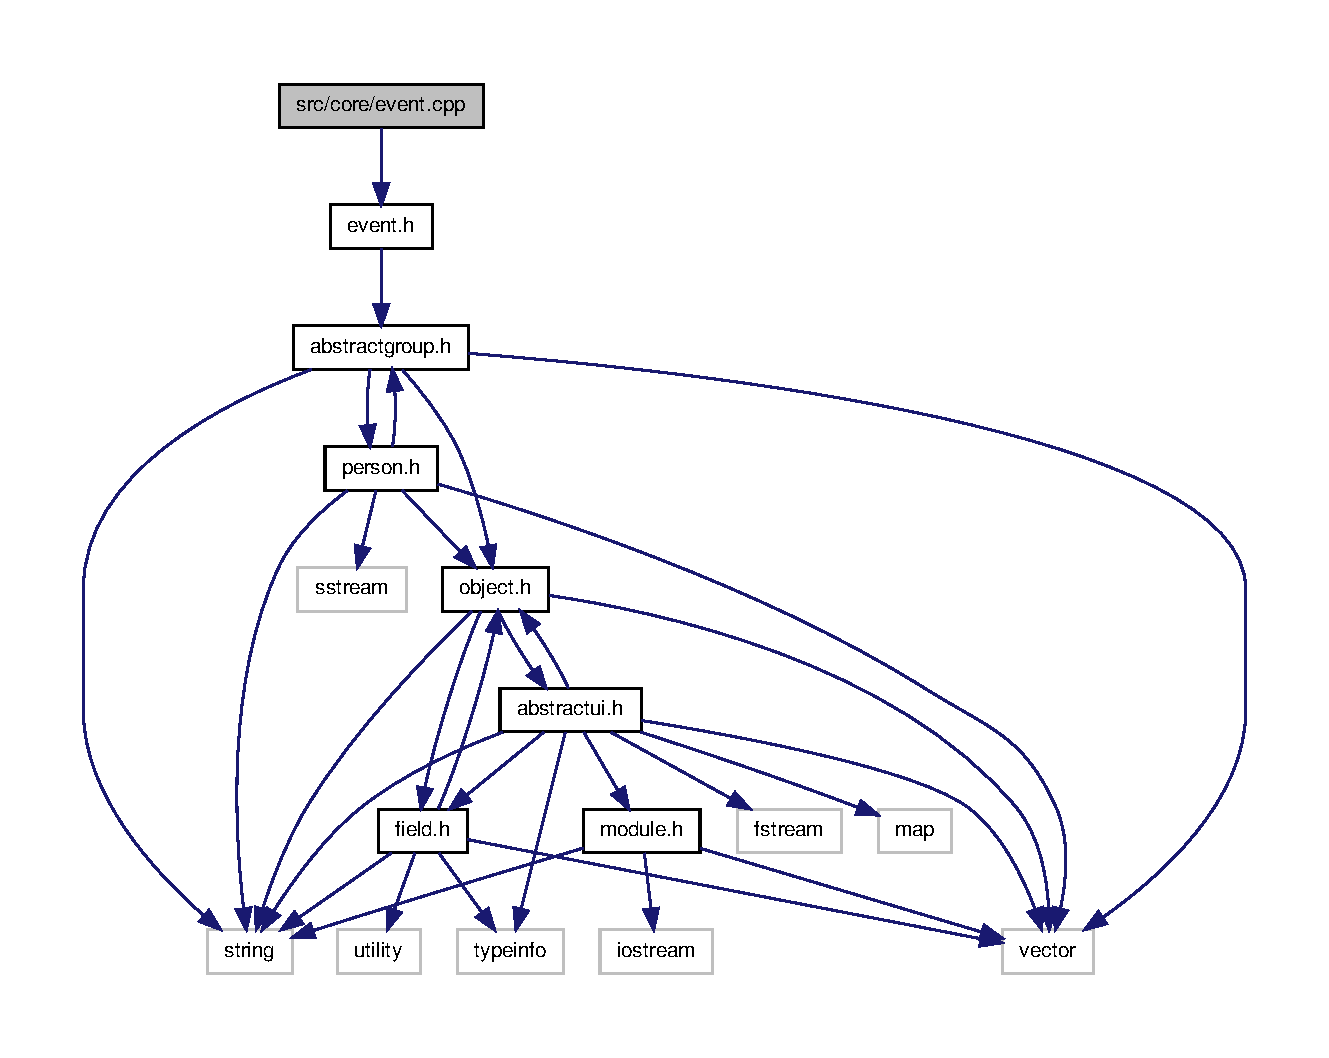
\includegraphics[width=400pt]{d6/d99/event_8cpp__incl}
\end{center}
\end{figure}

\hypertarget{event_8h}{
\section{src/event.h File Reference}
\label{dd/d20/event_8h}\index{src/event.h@{src/event.h}}
}
{\ttfamily \#include $<$string$>$}\par
{\ttfamily \#include $<$vector$>$}\par
{\ttfamily \#include $<$time.h$>$}\par
{\ttfamily \#include $<$types.h$>$}\par
{\ttfamily \#include $<$group.h$>$}\par
{\ttfamily \#include $<$person.h$>$}\par
{\ttfamily \#include $<$calendar.h$>$}\par
\subsection*{Classes}
\begin{DoxyCompactItemize}
\item 
class \hyperlink{classEvent}{Event}
\begin{DoxyCompactList}\small\item\em Class keeps information about event. \item\end{DoxyCompactList}\end{DoxyCompactItemize}

\hypertarget{group_8cpp}{
\section{src/core/group.cpp File Reference}
\label{d3/d97/group_8cpp}\index{src/core/group.cpp@{src/core/group.cpp}}
}
{\ttfamily \#include $<$group.h$>$}\par
Include dependency graph for group.cpp:
\nopagebreak
\begin{figure}[H]
\begin{center}
\leavevmode
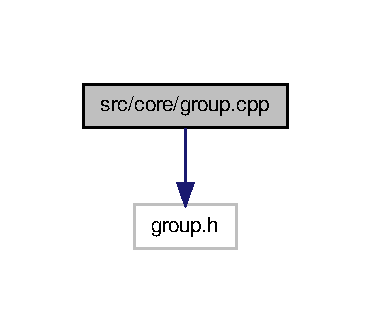
\includegraphics[width=178pt]{d0/dca/group_8cpp__incl}
\end{center}
\end{figure}

\hypertarget{group_8h}{
\section{src/group.h File Reference}
\label{d9/dd1/group_8h}\index{src/group.h@{src/group.h}}
}
{\ttfamily \#include $<$iostream$>$}\par
{\ttfamily \#include $<$string$>$}\par
{\ttfamily \#include $<$vector$>$}\par
{\ttfamily \#include \char`\"{}types.h\char`\"{}}\par
{\ttfamily \#include \char`\"{}group\_\-content.h\char`\"{}}\par
{\ttfamily \#include \char`\"{}calendar.h\char`\"{}}\par
{\ttfamily \#include \char`\"{}person.h\char`\"{}}\par
\subsection*{Classes}
\begin{DoxyCompactItemize}
\item 
class \hyperlink{classGroup}{Group}
\begin{DoxyCompactList}\small\item\em Class keeps information about group of people. \item\end{DoxyCompactList}\end{DoxyCompactItemize}

\hypertarget{group__content_8h}{
\section{src/group\_\-content.h File Reference}
\label{dc/db3/group__content_8h}\index{src/group\_\-content.h@{src/group\_\-content.h}}
}
{\ttfamily \#include $<$string$>$}\par
{\ttfamily \#include $<$group.h$>$}\par
{\ttfamily \#include $<$person.h$>$}\par
\subsection*{Classes}
\begin{DoxyCompactItemize}
\item 
struct \hyperlink{structGroup__Content__}{Group\_\-Content\_\-}
\end{DoxyCompactItemize}
\subsection*{Typedefs}
\begin{DoxyCompactItemize}
\item 
typedef struct \hyperlink{structGroup__Content__}{Group\_\-Content\_\-} \hyperlink{group__content_8h_ae838473c14b60b64e84dc69de8f2e594}{Group\_\-Content}
\end{DoxyCompactItemize}


\subsection{Typedef Documentation}
\hypertarget{group__content_8h_ae838473c14b60b64e84dc69de8f2e594}{
\index{group\_\-content.h@{group\_\-content.h}!Group\_\-Content@{Group\_\-Content}}
\index{Group\_\-Content@{Group\_\-Content}!group_content.h@{group\_\-content.h}}
\subsubsection[{Group\_\-Content}]{\setlength{\rightskip}{0pt plus 5cm}typedef struct {\bf Group\_\-Content\_\-}  {\bf Group\_\-Content}}}
\label{dc/db3/group__content_8h_ae838473c14b60b64e84dc69de8f2e594}

\hypertarget{main_8cpp}{
\section{src/main.cpp File Reference}
\label{df/d0a/main_8cpp}\index{src/main.cpp@{src/main.cpp}}
}
{\ttfamily \#include $<$iostream$>$}\par
{\ttfamily \#include $<$time.h$>$}\par
{\ttfamily \#include $<$vector$>$}\par
{\ttfamily \#include $<$types.h$>$}\par
{\ttfamily \#include $<$event\_\-template.h$>$}\par
{\ttfamily \#include $<$queue.h$>$}\par
{\ttfamily \#include $<$commands.h$>$}\par
{\ttfamily \#include $<$userinterface.h$>$}\par
{\ttfamily \#include $<$person.h$>$}\par
{\ttfamily \#include $<$group.h$>$}\par
{\ttfamily \#include $<$event.h$>$}\par
{\ttfamily \#include $<$data\_\-storage.h$>$}\par
{\ttfamily \#include $<$file\_\-storage.h$>$}\par
\subsection*{Functions}
\begin{DoxyCompactItemize}
\item 
int \hyperlink{main_8cpp_a0ddf1224851353fc92bfbff6f499fa97}{main} (int argc, char $\ast$argv\mbox{[}$\,$\mbox{]})
\end{DoxyCompactItemize}


\subsection{Function Documentation}
\hypertarget{main_8cpp_a0ddf1224851353fc92bfbff6f499fa97}{
\index{main.cpp@{main.cpp}!main@{main}}
\index{main@{main}!main.cpp@{main.cpp}}
\subsubsection[{main}]{\setlength{\rightskip}{0pt plus 5cm}int main (
\begin{DoxyParamCaption}
\item[{int}]{argc, }
\item[{char $\ast$}]{argv\mbox{[}$\,$\mbox{]}}
\end{DoxyParamCaption}
)}}
\label{df/d0a/main_8cpp_a0ddf1224851353fc92bfbff6f499fa97}

\hypertarget{person_8cpp}{
\section{src/person.cpp File Reference}
\label{d8/de5/person_8cpp}\index{src/person.cpp@{src/person.cpp}}
}
{\ttfamily \#include $<$person.h$>$}\par

\hypertarget{person_8h}{
\section{src/include/person.h File Reference}
\label{d4/d98/person_8h}\index{src/include/person.h@{src/include/person.h}}
}
{\ttfamily \#include $<$string$>$}\par
{\ttfamily \#include $<$sstream$>$}\par
{\ttfamily \#include $<$vector$>$}\par
{\ttfamily \#include $<$object.h$>$}\par
{\ttfamily \#include $<$abstractgroup.h$>$}\par
Include dependency graph for person.h:
\nopagebreak
\begin{figure}[H]
\begin{center}
\leavevmode
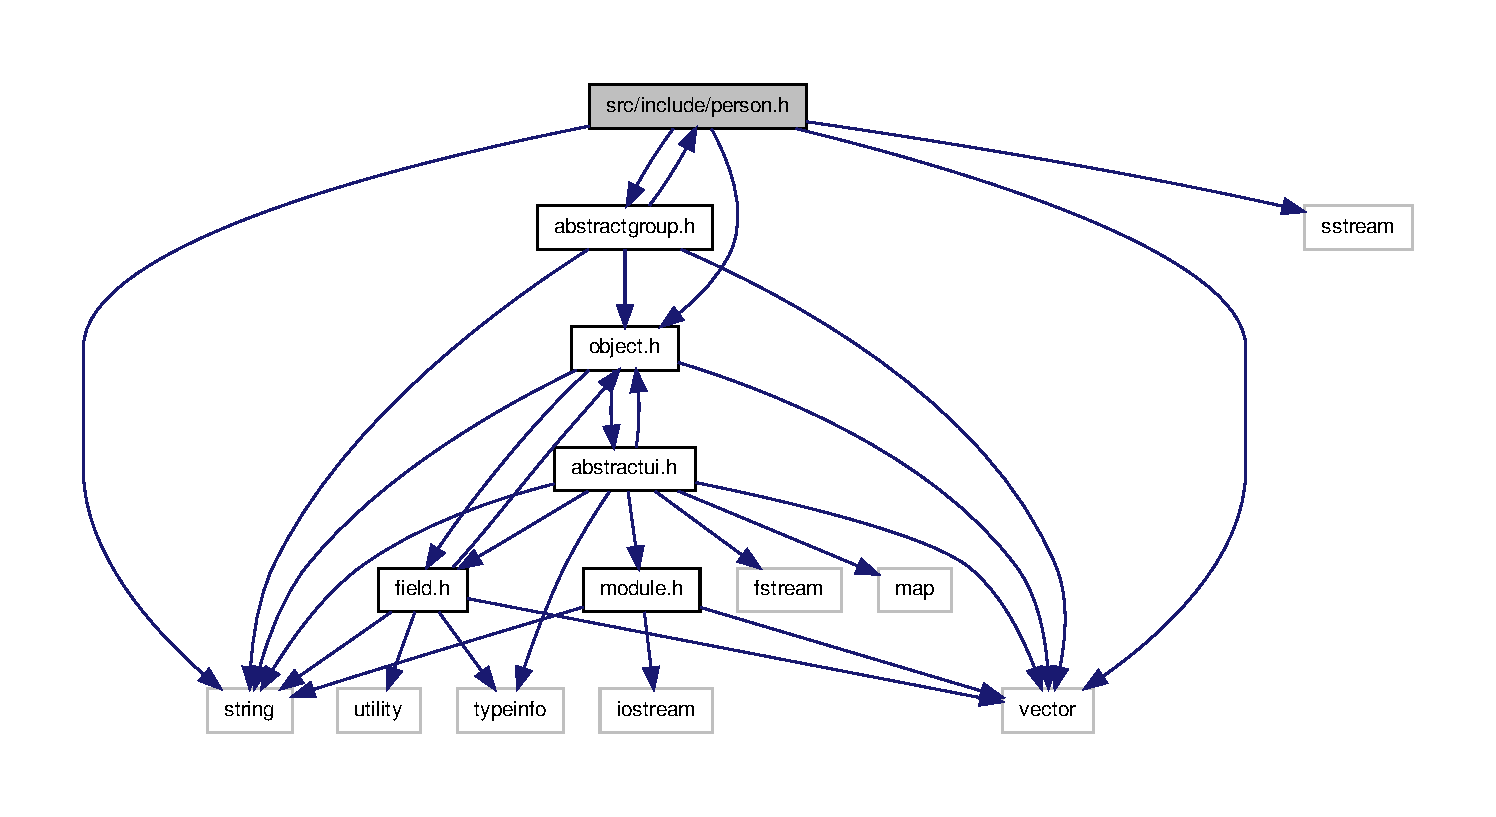
\includegraphics[width=400pt]{de/de3/person_8h__incl}
\end{center}
\end{figure}
This graph shows which files directly or indirectly include this file:
\nopagebreak
\begin{figure}[H]
\begin{center}
\leavevmode
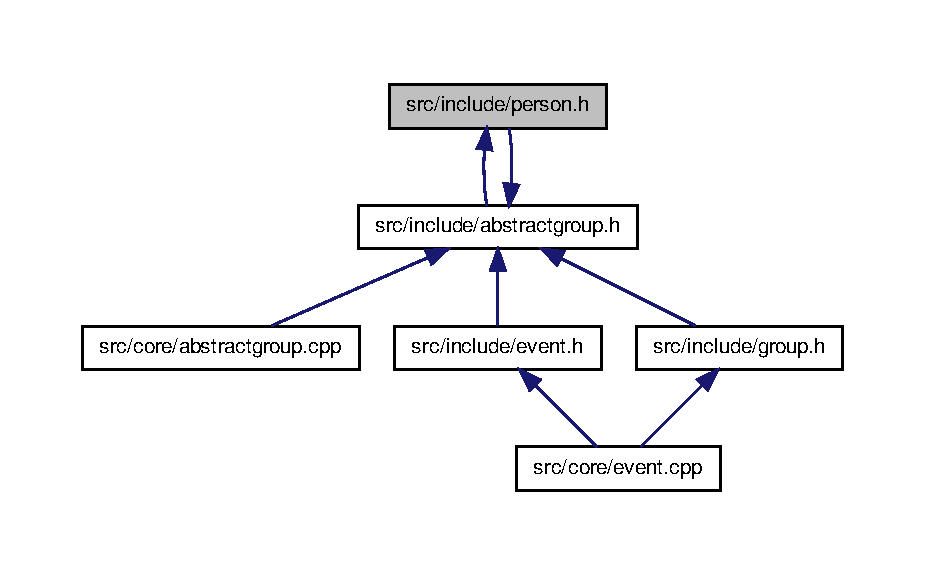
\includegraphics[width=400pt]{dc/daa/person_8h__dep__incl}
\end{center}
\end{figure}
\subsection*{Classes}
\begin{DoxyCompactItemize}
\item 
class \hyperlink{classCore_1_1Person}{Core::Person}
\begin{DoxyCompactList}\small\item\em Class keeps person unique data. \item\end{DoxyCompactList}\end{DoxyCompactItemize}
\subsection*{Namespaces}
\begin{DoxyCompactItemize}
\item 
namespace \hyperlink{namespaceCore}{Core}


\begin{DoxyCompactList}\small\item\em \hyperlink{namespaceCore}{Core} model classes. \item\end{DoxyCompactList}

\end{DoxyCompactItemize}

\hypertarget{types_8h}{
\section{src/types.h File Reference}
\label{d9/d49/types_8h}\index{src/types.h@{src/types.h}}
}
\subsection*{Typedefs}
\begin{DoxyCompactItemize}
\item 
typedef unsigned long long \hyperlink{types_8h_a0b60c08a3ab1435cccc5643d32d8ccee}{id\_\-type}
\item 
typedef struct \hyperlink{structGroup__Content__}{Group\_\-Content\_\-} \hyperlink{types_8h_abda815bcb63ee903900f16cef4d83cdc}{Group\_\-Content}
\end{DoxyCompactItemize}


\subsection{Typedef Documentation}
\hypertarget{types_8h_abda815bcb63ee903900f16cef4d83cdc}{
\index{types.h@{types.h}!Group\_\-Content@{Group\_\-Content}}
\index{Group\_\-Content@{Group\_\-Content}!types.h@{types.h}}
\subsubsection[{Group\_\-Content}]{\setlength{\rightskip}{0pt plus 5cm}typedef struct {\bf Group\_\-Content\_\-} {\bf Group\_\-Content}}}
\label{d9/d49/types_8h_abda815bcb63ee903900f16cef4d83cdc}
\hypertarget{types_8h_a0b60c08a3ab1435cccc5643d32d8ccee}{
\index{types.h@{types.h}!id\_\-type@{id\_\-type}}
\index{id\_\-type@{id\_\-type}!types.h@{types.h}}
\subsubsection[{id\_\-type}]{\setlength{\rightskip}{0pt plus 5cm}typedef unsigned long long {\bf id\_\-type}}}
\label{d9/d49/types_8h_a0b60c08a3ab1435cccc5643d32d8ccee}

\hypertarget{userinterface_8cpp}{
\section{src/userinterface.cpp File Reference}
\label{d4/dcb/userinterface_8cpp}\index{src/userinterface.cpp@{src/userinterface.cpp}}
}
{\ttfamily \#include \char`\"{}userinterface.h\char`\"{}}\par

\hypertarget{userinterface_8h}{
\section{src/userinterface.h File Reference}
\label{df/d52/userinterface_8h}\index{src/userinterface.h@{src/userinterface.h}}
}
{\ttfamily \#include $<$string$>$}\par
{\ttfamily \#include $<$vector$>$}\par
{\ttfamily \#include $<$time.h$>$}\par
{\ttfamily \#include $<$stdio.h$>$}\par
{\ttfamily \#include $<$types.h$>$}\par
{\ttfamily \#include $<$commands.h$>$}\par
{\ttfamily \#include $<$queue.h$>$}\par
{\ttfamily \#include $<$group\_\-content.h$>$}\par
{\ttfamily \#include $<$person.h$>$}\par
{\ttfamily \#include $<$group.h$>$}\par
{\ttfamily \#include $<$event.h$>$}\par
{\ttfamily \#include $<$calendar.h$>$}\par
{\ttfamily \#include $<$data\_\-storage.h$>$}\par
\subsection*{Classes}
\begin{DoxyCompactItemize}
\item 
class \hyperlink{classUserInterface}{UserInterface}
\begin{DoxyCompactList}\small\item\em Class provides user interface. \item\end{DoxyCompactList}\end{DoxyCompactItemize}
\subsection*{Enumerations}
\begin{DoxyCompactItemize}
\item 
enum \hyperlink{userinterface_8h_a5a0e707f53d6c5632b2fb5ffd2d22a11}{default\_\-format} \{ \hyperlink{userinterface_8h_a5a0e707f53d6c5632b2fb5ffd2d22a11af9c208c7d7a0f102f2683165540c882d}{ASCII}, 
\hyperlink{userinterface_8h_a5a0e707f53d6c5632b2fb5ffd2d22a11a0ace72efd9e987dfd807365d0ca50141}{DATE}
 \}
\end{DoxyCompactItemize}


\subsection{Enumeration Type Documentation}
\hypertarget{userinterface_8h_a5a0e707f53d6c5632b2fb5ffd2d22a11}{
\index{userinterface.h@{userinterface.h}!default\_\-format@{default\_\-format}}
\index{default\_\-format@{default\_\-format}!userinterface.h@{userinterface.h}}
\subsubsection[{default\_\-format}]{\setlength{\rightskip}{0pt plus 5cm}enum {\bf default\_\-format}}}
\label{df/d52/userinterface_8h_a5a0e707f53d6c5632b2fb5ffd2d22a11}
\begin{Desc}
\item[Enumerator: ]\par
\begin{description}
\index{ASCII@{ASCII}!userinterface.h@{userinterface.h}}\index{userinterface.h@{userinterface.h}!ASCII@{ASCII}}\item[{\em 
\hypertarget{userinterface_8h_a5a0e707f53d6c5632b2fb5ffd2d22a11af9c208c7d7a0f102f2683165540c882d}{
ASCII}
\label{df/d52/userinterface_8h_a5a0e707f53d6c5632b2fb5ffd2d22a11af9c208c7d7a0f102f2683165540c882d}
}]ASCII Time format. \index{DATE@{DATE}!userinterface.h@{userinterface.h}}\index{userinterface.h@{userinterface.h}!DATE@{DATE}}\item[{\em 
\hypertarget{userinterface_8h_a5a0e707f53d6c5632b2fb5ffd2d22a11a0ace72efd9e987dfd807365d0ca50141}{
DATE}
\label{df/d52/userinterface_8h_a5a0e707f53d6c5632b2fb5ffd2d22a11a0ace72efd9e987dfd807365d0ca50141}
}]Date Time format. \end{description}
\end{Desc}


\printindex
\end{document}
